\begin{summary}
First, new picking/weighting methods developed here and previously published
picking/weighting methods are compiled together to generate 168 different
paleomagnetic APWPs. Then, the APWP similarity measuring tool is used to find
which method\(s\) is$(are)$ good or bad. The final results tell us that the
``Age Position Picking (APP)'' method is better than the ``Age Mean Picking
(AMP)'' method for making a reliable paleomagnetic APWP and weighting is
actually unnecessary.
\end{summary}

\begin{keywords}
  Moving Average \textendash{} Weighting \textendash{} APWP \textendash{}
  Paleomagnetism.
\end{keywords}

\section{Introduction}

APWPs are generated by combining paleomagnetic poles for a particular rigid
block over the desired age range to produce a smoothed path. See the
Supplementary Material for some examples how the pole datasets are constrained
first.

\subsection{Not All Data Are Created Equal}

However, uncertainties in the age and location of paleomagnetic poles can vary
greatly for different poles.

\subsubsection{Age Error}

Although remanent magnetizations are generally assumed to be primary, many
events can cause remagnetisation (in which case the derived pole is `younger'
than the rock). If an event that has occurred since the rock's formation that
should affect the magnetisation (e.g., folding, thermal overprinting due to
intrusion) can be shown to have affected it, then it constrains the
magnetisation to have been acquired before that event. Recognising or ruling
out remagnetisations depends on these field tests, which are not always
performed or possible. Even a passed field test may not be useful if field test
shows magnetisation acquired prior to a folding event tens of millions of years
after initial rock formation.

The most obvious characteristic we can observe from paleomagnetic data is that
some poles have very large age ranges, e.g., more than 100 Myr. The
magnetization age should be some time between the information of the rock and
folding events. There are also others where we have similar position but the age
constraint is much narrower, e.g. 10 Myr window or less. Obviously the latter
kind of data is more valuable than the one with large age range.

\subsubsection{Position Error}

The errors of pole latitudes and longitudes are 95\% confidence ellipses, which
also vary greatly in magnitude. All paleomagnetic poles have some associated
uncertainties due to measurement error and the nature of the geomagnetic field.
More uncertainties can be added by too few samples, sampling spanning too short
a time range to approximate a GAD field, failure to remove overprints during
demagnetisation, etc.

\subsubsection{Data Consistency}

Paleomagnetic poles of a rigid plate or block should be continuous time series.
For a rigid plate, two poles with similar ages shouldn't be dramatically
different in location. Sometimes, this is the case. Sometimes we have further
separated poles with close ages.

There are a number of possible causes for these outliers, including:

\verb"Lithology"

For poor consistency of data, it is potentially because of different
inclinations or declinations. The first thing we should consider about is their
lithology. We want to check if the sample rock are igneous or sedimentary,
because sediment compaction can result in anomalously shallow
inclinations~\cite{T18}. In addition, we also can check if the rock are redbeds
or non-redbeds. Although whether redbeds record a detrital signal or a later
Chemical Remanent Magnetization (CRM) is still somewhat controversial, both
sedimentary rocks and redbeds could lead to inconsistency in direction compared
to igneous rocks.

\verb"Local Rotations"

Local deformation between two paleomagnetic localities invalidates the rigid
plate assumption and could lead to inconsistent VGP directions. So if
discordance is due to local deformation, and we would ideally want to exclude
such poles from our APWP calculation.

\verb"Other Factors"

In most cases, mean pole age (centre of age error) has just been binned. If
any of the poles have large age errors, they could be different ages from each
other and sample entirely different parts of the APWP\@. Conversely, if any of
the poles have too few samples, or were not sampled over enough time to average
to a GAD field, a discordant pole may be due to unreduced secular variation.

\subsubsection{Data Density}

As we go back in time, we have lower quality and lower density (or quantity) of
data, for example, the Precambrian or Early Paleozoic paleomagnetic data are
relatively fewer than Middle-Late Phanerozoic ones, and most of them are not
high-quality, e.g., larger errors in both age and location. The combination of
lower data quality with lower data density means that a single `bad' pole (with
large errors in age and/or location) can much more easily distort the
reconstructed APWP, because there are few or no `good' poles to counteract its
influence.

Data density also varies between different plates. E.g., we have a relatively
high density of paleomagnetic data for North American Craton (NAC), but few
poles exist for Greenland and Arabia. Based on mean age (mean of lower and upper
magnetic ages), for 120\textendash0 Ma, the \textbf{Global Paleomagnetic
Database} (GPMDB) version 4.6b~\cite{P05} has more than 130 poles for NAC, but
only 17 for Greenland and 24 for Arabia.

\subsubsection{Publication Year}

The time when the data was published should also be considered, because
magnetism measuring methodology, technology and equipments have been improved
since the early 20th century. For example, stepwise demagnetisation, which is
the most reliable method of detecting and removing secondary overprints, has
only been in common use since the mid 1980s.

In summary, not all paleomagnetic poles are created equal, which leads to an
important question: how to best combine poles of varying quality into a coherent
and accurate APWP\@?

\subsection{Existing Solutions and General Issues}

Paleomagnetists have proposed a variety of methods to filter so-called ``bad''
data, or give lower weights to those ``bad'' data before generating an APWP,
e.g., two widely used methods: the V90 reliability criteria~\cite{v90} and the
BC02 selection criteria provided by Besse \& Courtillot \shortcite{B02}.
Briefly, the V90 criteria for paleomagnetic results includes seven criteria: (1)
Well determined age; (2) At least 25 samples with Fisher~\cite{F53} precision
$\kappa$ greater than 10 and $\alpha95$ less than 16\degree; (3) Detailed
demagnetisation results reported; (4) Passed field tests; (5) Tectonic coherence
with continent and good structural control; (6) Identified antipodal reversals;
(7) Lack of similarity with younger poles~\cite{T92}. The total criteria
satisfied (0\textendash7) is then used as a measure of a paleomagnetic result's
overall reliability, which is known as Q (quality) factor~\cite{T92}. Q factor
is indeed a very straightforward way to get a quantitalized reliability score.
Also it then can be conveniently used in the later calculations of
APWPs~\cite{T92}. But at the same time this is a fairly basic filter that lumps
together criteria that may not be equally important. Compared with V90, the BC02
criteria suggests stricter filtering, e.g., using only poles with at least 6
sampling sites and 36 samples, each site having $\alpha95$ less than 10\degree\
in the Cenozoic and 15\degree\ in the Mesozoic. B02 is also straightforward and
convenient to use, but some useful data may be filtered out and wasted
especially for a period where there are only limited number of data. In
addition, there has been limited study of how effective these marking/filtering
methods are at reconstructing a `true' APWP, and for most studies after a basic
filtering of `low quality' poles, the remaining poles are, in fact, treated
equally.

Above all, there haven't been any real attempts to study how APWP fits may be
improved by filtering/weighting data. This paper is presented to address these
issues.


\section{Methods}

For most of Earth history, concretely for times before c. 170 Ma, the age of the
oldest magnetic anomaly identification, paleomagnetism is the only accepted
quantitative method for reconstructing plate motions and past paleogeographies.
After about 170 Ma, multiple data sources can help constrain plate motions in
more accurate ways. One of the most developed and studied plate kinematics
models is the Fixed Hotspot Model (FHM)~\cite{M93,M99}, which assumes the
Atlantic and Indian hotspots are relatively fixed. Another one is the Moving
Hotspot Model (MHM)~\cite{O05}, which is based on mantle convection models that
indicate large motions of the Indo-Atlantic hotspots.

\subsection{Reference Paths: The Hotspot and Seafloor Spreading Model Predicted}

Such a model like FHM or MHM can predict APWPs for main continents, e.g.\ the
North America (Plate ID 101) (Fig.~\ref{fig-fhsPred} and
Fig.~\ref{fig-mhsPred}), the India (501) (Fig.~\ref{fig-fhsPred501} and
Fig.~\ref{fig-mhsPred501}) and the Australia (801) (Fig.~\ref{fig-fhsPred801}
and Fig.~\ref{fig-mhsPred801}), with the help of global tectonic plate motion
data (i.e.\ plate circuits) from the ocean basins (i.e.\ spreading sea floors)
that has been reconstructed for the last c. 180\textendash200 Myr (although the
extrapolation is required; hard to constrain uncertainties). These more accurate
and totally different-source derived model-predicted APWPs can be compared to
data from the paleomagnetic database. For about 120 Ma to the present, India
drifts much faster than North America and Australia. North America has been
drifting rather slow. Australia's drifting rate is between North America and
India. In addition, India drifts almost north, whereas North America east and
then north, and Australia west and then north. So these three continents are
representatives for three different types of plate kinematics.

The oldest pole that can be predicted from the FHM is about 120 Ma. For example,
the North American 120\textendash0 Ma APWP predicted from this rotation model
and latest published spreading ridge rotations (collected plate circuit data
will be shared as a supplementary material) will be taken as a reference path
(Fig.~\ref{fig-fhsPred}), which will be compared with paleomagnetic APWPs for
the same plate or continent.

\begin{figure*}
\centering
\includegraphics[width=1.01\textwidth]{figures/fhs.pdf}
\caption[120\textendash0 Ma FHM predicted APWP of North America]{FHM
predicted 120\textendash0 Ma APWP for $NAC$ through the North
America\textendash{}Nubia\textendash{}Mantle plate circuit. Its age step is 5
Myr.}\label{fig-fhsPred}
\end{figure*}

\begin{figure*}
\centering
\includegraphics[width=1.01\textwidth]{figures/mhs.pdf}
\caption[120\textendash0 Ma MHM predicted APWP of North America]{MHM
predicted 120\textendash0 Ma APWP for $NAC$ through the North
America\textendash{}Nubia\textendash{}Mantle plate circuit. Its age step is 5
Myr. The dashed line is the FHM predicted path shown in
Fig.~\ref{fig-fhsPred} without confidence ovals for clarity.}\label{fig-mhsPred}
\end{figure*}

\begin{figure*}
\centering
\includegraphics[width=1.01\textwidth]{figures/fhs501.pdf}
\caption[120\textendash0 Ma FHM predicted APWP of India]{FHM predicted
120\textendash0 Ma APWP for India through the
India\textendash{}Somalia\textendash{}Nubia\textendash{}Mantle plate circuit.
Its age step is 5 Myr.}\label{fig-fhsPred501}
\end{figure*}

\begin{figure*}
\centering
\includegraphics[width=1.01\textwidth]{figures/mhs501.pdf}
\caption[120\textendash0 Ma MHM predicted APWP of India]{MHM predicted
120\textendash0 Ma APWP for India through the
India\textendash{}Somalia\textendash{}Nubia\textendash{}Mantle plate circuit.
Its age step is 5 Myr. The dashed line is the FHM predicted path shown in
Fig.~\ref{fig-fhsPred501} without confidence ovals for
clarity.}\label{fig-mhsPred501}
\end{figure*}

\begin{figure*}
\centering
\includegraphics[width=1.01\textwidth]{figures/fhs801.pdf}
\caption[120\textendash0 Ma FHM predicted APWP of Australia]{FHM predicted
120\textendash0 Ma APWP for Australia through the Australia\textendash{}East
Antarctica\textendash{}Somalia\textendash{}Nubia\textendash{}Mantle plate
circuit. Its age step is 5 Myr.}\label{fig-fhsPred801}
\end{figure*}

\begin{figure*}
\centering
\includegraphics[width=1.01\textwidth]{figures/mhs801.pdf}
\caption[120\textendash0 Ma MHM predicted APWP of Australia]{MHM predicted
120\textendash0 Ma APWP for Australia through the Australia\textendash{}East
Antarctica\textendash{}Somalia\textendash{}Nubia\textendash{}Mantle plate
circuit. Its age step is 5 Myr. The dashed line is the FHM predicted path shown
in Fig.~\ref{fig-fhsPred801} without confidence ovals for
clarity.}\label{fig-mhsPred801}
\end{figure*}

\subsection{120\textendash0 Ma Paleomagnetic APWPs}

The GPMDB 4.6b~\cite{P05}, data source used here, includes 9514 paleopoles for
ages of 3,500 Ma to the present published from 1925 to 2016. A polygon can be
drawn around a set of data, whose sampling sites we believe belong to a specific
plate or rigid block. Then the {\em Spatial Join\/} technique~\cite{J07} helps
join attributes from the polygon to the paleomagnetic data based on the spatial
relationship allowing data within this polygon to be extracted from the whole
raw large dataset without splitting a subset just for a specific plate. That
allows us to quickly select subsets of the database based on geographic
constraints just as easily as for age. Of course, the boundary of this polygon
must be reasonably along a tectonic boundary (see the details about data
filtering for North America in the Supplementary Material). The temporal
distributions of North American, Indian and Australian 120\textendash0 Ma poles
are shown in Fig.~\ref{fig-120NAhist}, Fig.~\ref{fig-120INhist} and
Fig.~\ref{fig-120AUhist}. Compared with North American and Australian
paleomagnetic paleo-poles, Indian paleomagnetic paleo-poles are in relatively
lower density in general except during the period of about 60\textendash70 Ma
(Fig.~\ref{fig-120INhist}).

\begin{figure*}
\centering
\includegraphics[width=.9\textwidth]{figures/120NAhist.pdf}
\caption[Distribution of 120\textendash0 Ma North American poles]{Temporal
distribution of 120\textendash0 Ma $NAC$ (101) paleomagnetic poles in 10 Myr
binning and 5 Myr step. For distribution a, each bin only counts in the
midpoints of pole error bars (not including those right at bin edges); For
distribution b, as long as the bar intersects with the bin (not including those
intersecting only at one of bin edges), it is counted in. Inside the
parentheses, i means igneous rocks derived (red bars), r means sedimentary rocks
with redbeds involved derived (orange bars), and m means metamorphic-dominated
rocks derived (blue bars); the left are pure sedimentary rocks derived (black
bars). The midpoints published not later than 1983 are black-dotted.}\label{fig-120NAhist}
\end{figure*}

\begin{figure*}
\centering
\includegraphics[width=.91\textwidth]{figures/120INhist.pdf}
\caption[Distribution of 120\textendash0 Ma Indian poles]{Temporal distribution
of 120\textendash0 Ma Indian (501) paleomagnetic poles. See
Fig.~\ref{fig-120NAhist} for more information.}\label{fig-120INhist}
\end{figure*}

\begin{figure*}
\centering
\includegraphics[width=.91\textwidth]{figures/120AUhist.pdf}
\caption[Distribution of 120\textendash0 Ma Australian poles]{Temporal
distribution of 120\textendash0 Ma Australian (801) paleomagnetic poles. See
Fig.~\ref{fig-120NAhist} for more information.}\label{fig-120AUhist}
\end{figure*}

\subsection{Picking Data for A Certain Time Window}

\subsubsection{Moving Average}

The moving average method, also called ``running mean'' or ``moving
window''~\cite{T08} method, calculates the average of values between a certain
data (age in our case) range; the average is then recalculated as the limits of
the bin are repeatedly incremented upwards. In addition to the traditional
moving windows averaging algorithm, a newly developed moving average method is
also used, referred to here as the ``Age Position Picking (APP)'' method. The
difference of this moving average method from the one built in
GMAP~\cite{T99,T08} is that the whole magnetic age range is taken into account
in each window, while GMAP only considers the mid-point of the low and high
magnetic age of each pole, an algorithm referred to as the ``Age Mean Picking
(AMP)'' method.

Normally each paleo-pole in the paleomagnetic database is treated as a point
with an age that is the mid-point between the upper and lower age limits, i.e.
AMP, but this is problematic for paleomagnetic data with large age ranges
(especially if they turn out to be primary magnetization that should plot at old
end of age range). We are trying a method, APP, that includes a paleo-pole in
the moving average bin if any part of its specified age range falls within that
bin. If, for example, we have a pole which is constrained to within 10 and 20 Ma
of age, and we have a 2 Myr moving window with a 1 Myr age step, then it
shouldn't just be in the 14\textendash16 Ma bin (for the mid-point age of 15
Ma)\textemdash{}it should be in the 9\textendash11,10\textendash12,
11\textendash13,12\textendash14\ldots17\textendash19,18\textendash20, and
19\textendash21 Ma bins. So the average poles are produced from each bin, and
each original pole is represented over its entire possible acquisition age.
Fig.~\ref{fig-nac-maplat} shows an example of moving average with a 10 Myr
window and a 5 Myr step. So, for example, for the window of 15 Ma to 5 Ma (the
light blue bin in Fig.~\ref{fig-nac-maplat}), the AMP method calculates the
Fisher mean pole of only 5 poles, while the APP method calculates the mean pole
of 9 poles. From comparison of mean poles of the picked poles for the light blue
age window with the two different algorithms (the 10 Ma mean poles in
Fig.~\ref{fig-fhsPred}), the mean pole from the APP method is closer to the 10
Ma pole in the FHM predicted path, which indicates more data diluting the effect
of outliers.

\begin{figure*}
\centering
\includegraphics[width=1.01\textwidth]{figures/binning.pdf}
\caption[Moving average (MA) methods]{An example of 10 Myr moving window and 5
Myr step in the moving average method, based on poles of the $NAC$. Every age
window has a different color. Red points are the midpoints of low and high
magnetic ages. The vertical axis has no specific meaning here.
}\label{fig-nac-maplat}
\end{figure*}

In addition, technically we don't want to let the step length more than the
window length, in which cases we would lose data between windows.

\paragraph{Picking}

The 28 picking methods include AMP, APP and also those with filtering or
corrections implemented onto the two (Table.~\ref{tab-pick}).

\begin{table}
\centering
\caption{List of all Picking (i.e. Binning) algorithms developed in this paper.
         AMP, Age Mean Picking (See Section ``Moving Average''); APP, Age
         Position Picking.}\label{tab-pick}
\begin{tabular}{@{}ll@{}}
\toprule
No. & Picking Algorithm \\ \midrule
0 & AMP \\
1 & APP \\
2 & AMP (``$\alpha$95/Age range'' no more than ``15/20'') \\
3 & APP (``$\alpha$95/Age range'' no more than ``15/20'') \\
4 & AMP (mainly or only igneous) \\
5 & APP (mainly or only igneous) \\
6 & AMP (contain igneous and not necessarily mainly) \\
7 & APP (contain igneous and not necessarily mainly) \\
8 & AMP (unflatten sedimentary) \\
9 & APP (unflatten sedimentary) \\
10 & AMP (nonredbeds) \\
11 & APP (nonredbeds) \\
12 & AMP (unflatten redbeds) \\
13 & APP (unflatten redbeds) \\
14 & AMP (published after 1983) \\
15 & APP (published after 1983) \\
16 & AMP (published before 1983) \\
17 & APP (published before 1983) \\
18 & AMP (exclude commented local rot or secondary print) \\
19 & APP (exclude commented local rot or secondary print) \\
20 & AMP (exclude local rot or correct it if suggested) \\
21 & APP (exclude local rot or correct it if suggested) \\
22 & AMP (filtered using SS05 palaeomagnetic reliability criteria) \\
23 & APP (filtered using SS05 palaeomagnetic reliability criteria) \\
24 & AMP (exclude superseded data already included in other results) \\
25 & APP (exclude superseded data already included in other results) \\
26 & AMP (comb of 22 and 24) \\
27 & APP (comb of 23 and 25) \\ \bottomrule
\end{tabular}
\raggedright{Notes: SS05,~\cite{S05}}
\end{table}

\subparagraph{Filtering through $\alpha$95 and Age Range}

For this specific filter, the poles are picked out through setting $\alpha$95 of
$\leq15\degree$ and age uncertainty of $\leq20$ Myr.

\subparagraph{Filtering Out Non-igneous Derived Poles}

With this filter, the poles are mainly or only from igneous rocks with extrusive
or intrusive type.

\subparagraph{Filtering Out Igneous Unrelated Poles}

With this filter, the poles are from rocks that contain extrusive or intrusive
igneous type. In other words, the rock type could be mainly sedimentary or
metamorphic.

\subparagraph{Inclination Shallowing and Unflattening}

To test if unflattening possible inclination shallowing in sedimentary rocks can
improve the APWP fitting outcomes, the flattening function~\cite{K55} $\tan I_o
= f \tan I_f$ is used to unflatten assumed existing inclination shallowing in
sedimentary-based or redbeds-based paleomagnetic data (No $5$ and $7$ in
Table.~\ref{tab-pick}), where $I_o$ is the observed inclination, $I_f$ is the
unflattened inclination, and $f$ is the flattening factor (or shallowing
coefficient) ranging from unity (no flattening) to 0 (completely flattened).
Here $f=0.6$ is used in our calculations, according to the previous
experience~\cite{T12}.

\subparagraph{Filtering Out Poles Related to Red-beds}

Bias toward shallow inclinations is also observed in paleomagnetic data derived
from red-beds~\cite{T04}. For this filter, the poles derived from red-beds are
simply removed.

\subparagraph{Filtering Out Poles Published Earlier or Later}

It is also worthy to see if recently published data is able to produce a more
reliable APWP than relatively older data. Here 1983 is chosen as the division,
because the mean of the data publication years is about 1983.

\subparagraph{Filtering Out Poles Influenced by Local Rotations or Secondary
Print}

Some publications of paleomagnetic data suggest the data has probably been
affected by local rotations or secondary overprints. So for this filter, this
type of data are removed.

\subparagraph{Filtering Out Poles Influenced by Local Rotations or Correcting
Them if Suggested}

Some publications suggest the data has been through local rotation and propose a
solution of correction. With this filter, if there is a correction suggestion,
the data is corrected; if no, the data is simply removed.

\subparagraph{Filtering Using SS05 Liability Criteria}

SS05~\cite{S05} provided their criteria of picking paleomagnetic data for
producing their APWPs. This filter is reproducing their criteria by setting
$\alpha$95 of $\leq15\degree$, age uncertainty of $\leq40$ Myr, sampling sites'
quantity of $\geq4$, samples' quantity of at least 4 times of the sites, and
laboratory analytical procedure code of at least 2.

\subparagraph{Filtering Out Superseded Data}

In this filter, those superseded data already included in other newer results
are excluded.

\paragraph{Weighting}

Because all data is not created equal, we want to calculate a weighted mean pole
for a time interval with `better' (more likely to be reliable) poles counting
more than `worse'. For example, a pole with small $\alpha$95 and very well
constrained age is more likely to reflect APWP position at the selected age
point than a pole with large $\alpha$95 and very broad age range. There are many
potential ways to weight this data set which can obviously greatly influence the
final result, and we want to test this.

Six weighting algorithms (Table.~\ref{tab-weit}) have currently been developed
or reproduced according to published work to give different weights to data with
different qualities.

\begin{table}
\centering
\caption{List of all weighting algorithms developed in this
         paper.}\label{tab-weit}
\begin{tabular}{@{}ll@{}}
\toprule
No. & Weighting Algorithm \\ \midrule
0 & None \\
1 & Numbers of sites (B), Observations (N) \\
2 & Age uncertainty \\
3 & $\alpha$95 \\
4 & Age error Position to bin \\
5 & comb of 3 and 4 \\ \bottomrule
\end{tabular}
\end{table}

In order to average errors in orientation of the samples and scatter caused by
secular variation, a ``sufficient'' number of individually oriented samples
(observations) from ``enough'' sites must be satisfied~\cite{T18,v90,B02}. So
for the ``Numbers of sites (B), Observations (N)'' weighting (No $1$ in
Table.~\ref{tab-weit}), larger B and N mean stronger weighting. Through knowing
the pattern of all B and N in the database, the proposed solutions are as
follows. If both B and N are more than 1, weight=$(1- \frac{1}{B})*(1-
\frac{1}{N})$. There are data in GPMDB with only the number of sampling sites
(at least greater than 1) given, but no number of samples or only one sample
given, so for this case, if B$>$1 and N $\leq$ 1, weight=$(1- \frac{1}{B})*0.5$.
If only the number of samples (at least greater than 1) is given, and the
number of sampling sites is missing or only one, i.e. B$\leq$ 1 and N$>$1,
weight=$(1- \frac{1}{N})*0.5$. If B $\leq$ 1 and N $\leq$ 1 (there are only 23
datasets for the whole GPMDB 4.6b, including 18 with both B and N informations
missing), weight=0.2.

As for the ``Age uncertainty'' weighting (No $2$ in Table.~\ref{tab-weit}), a
well-constrained age should be known to within a half of a geological period
(e.g., Quaternary, Neogene, Triassic) for Phanerozoic data~\cite{v90,T18}.
Generally, this work follows this principle. However, for the periods of
Paleogene, Cretaceous, and Jurassic, their halves are all beyond a time span of
at least 20 Myr, which is relatively large for these relatively young geologic
periods. So for these three periods, a tighter age constraint is set using age
uncertainties of $\leq15$ Myr. So, for example, for NAC's Neogene
(23.03\textendash2.58 Ma according to GSA Geologic Time Scale) data, if age
uncertainty (the high magnetic age $-$ the low magnetic age) $\leq$ 10.225 (from
0.5* (23.03$-$2.58)) Myr, its weight = 1; if age uncertainty $>$ 10.225 Myr, its
weight = 10.225 / (high magnetic age $-$ low magnetic age). For the periods
spanning Jurassic to Paleogene, if age uncertainty $\leq15$ Myr, it get its
weight of 1; if age uncertainty $>15$ Myr, a weight of 15 / (high magnetic age
$-$ low magnetic age) is assigned instead.

For the ``$\alpha$95'' weighting (No $3$ in Table.~\ref{tab-weit}), smaller
radius of circle of 95\% confidence about mean remanence direction means less
error, so should get larger weight. Here, weight is from a Gaussian distribution
centered on 0 with standard deviation of 10, i.e., when $\alpha$95 $=$ 0,
weight=1; when $\alpha$95$>$0, weight$<$1. It is also worthwhile to mention that
if samples, where two poles are derived, are exactly from the same place and
same rock, and one $\alpha$95 is completely inside the other $\alpha$95, a zero
is assigned as the weight of the data with the larger $\alpha$95. Here, the same
procedure can be applied on A95 (circle of 95\% confidence about mean pole)
instead of $\alpha$95.

For the ``Age error Position to window'' weighting (No $4$ in
Table.~\ref{tab-weit}), if window intersects with young/old end of age bracket
or whole window overlaps with a part of age range, weight= (overlapping part)
/ (age range width); if whole age range is within window, weight= (window width)
/ (age range width) (note that when weight $>1$, it is set back to 1).

The ``Age error Position to window, and $\alpha$95'' weighting (No $5$ in
Table.~\ref{tab-weit}), is a combination of No $3$ (but here the standard
deviation is 15 though) and No $4$.

Some of the picking (Table.~\ref{tab-pick}) and weighting
(Table.~\ref{tab-weit}) methods developed here are also connected with the V90 Q
factors mentioned above. For example, Pt 2, 3 and Wt 2, 4, 5 are related to the
V90 criteria 1; Pt 2, 3, 22, 23, 26, 27 and Wt 1, 3 are related to the V90
criteria 2; Pt 22 and 23 are related to the V90 criteria 3; The data
constraining described in the Supplementary Material is related to the V90
criteria 5; and Pt 18 and 19 are related to the V90 criteria 7.

\subsection{Path Comparison Method}

Except the path comparison method (referred to as Measure 1 in the following
text) that has been detailedly described in Chapter 2, here is another
comparison method (referred to as Measure 2 in the following text) developed
originally.

First, the definition of the significant spatial difference $d_s$ is changed
into the fraction of $\mathbf{n}$ coeval pole pairs that are statistically
distinguishable from each other, as determined by a test for a common mean
direction. Then for the other two shape metrics $d_a$ and $d_l$, there is no
significance testing on them. The way of combining them three into the final
composite path difference is still the same.

It will be interesting to see if there is any difference between the results
given by these two methods. So we will have them both tested in the following
content.

\section{Results and Discussions}

\subsection{Results}

Is there any common pattern of the similarities for all the three continents?
First, the best and worst methods need to be determined. Here, the difference
values less than the one-standard-deviation interval (containing about 68.269\%
of the data values) are picked out as the ``best'' ones (lower about 15.866\% of
the data values), more than the one-standard-deviation interval as the ``worst''
ones (upper about 15.866\%). Then we will see if there is one method or several
methods labeled as ``best'' or ``worst'' for all the three continents.

\subsubsection{When FHM and Global Plate Tectonic Circuits Predicted APWP as
Reference}

First, we focus on analysing the results with FHM and global plate circuits
predicted APWP (Fig.~\ref{fig-fhsPred}, Fig.~\ref{fig-fhsPred501},
Fig.~\ref{fig-fhsPred801}) as the reference path.

\paragraph{10 Myr Binning and 5 Myr Stepping}

\subparagraph{Measure 1: Both Space and Shape Tested}

According to the results (Fig.~\ref{fig-dif} and Fig.~\ref{fig-d-dif}), we can
observe:
%
\begin{enumerate}
  \item the groups of picking-method-no 19 (APP with commented local-rotation or
        secondary-print studies excluded) and 21 (APP with local rotation
        excluded or corrected as suggested in the original sources)
        (Table.~\ref{tab-pick}) are among the best ones for all the three
        continents, while the groups of picking-method-no 2 (AMP with
        ``$\alpha$95/Age range'' no more than ``15\degree/20 Myr'') and 16 (AMP
        with only earlier-than-1983 studies), (Table.~\ref{tab-pick}) are among
        the worst for all them three.
  \item for both North America (101) and Australia (801), the groups of
        picking-method-no 1, 11, 13, 19, 21 and 25 (Table.~\ref{tab-pick}) are
        the best, and 2, 14, 16, 22 and 26 the worst. For both North America
		(101) and India (501), the groups of picking-method-no 4, 5, 7, 19 and
		21 are the best, and 2, 8, 16 and 18 the worst. For both India (501)
		and Australia (801), the best 19, 21 and the worst 2, 16 are the same as
		the ones for all the three continents as above-mentioned. These results
		also further indicate that APP methods generally produce better
		similarity than AMP methods, however, the picking-method-no 4 is
		special, which is one of the AMP methods but also one of the best for
		both North America and India.
  \item the results of North America (101) and Australia (801) are closer
		(Fig.~\ref{fig-d-dif}).
  \item For North America and India, newer studies (later than 1983) give
		better results, whereas for Australia older studies (before 1983) give
		better results, mainly because the number of older studies (65;
		Fig.~\ref{fig-au-dif}) is much greater than the number of newer studies
		(27).
  \item Weighting influences more to APP than AMP, especially for the cases
		when there are plenty of paleo-poles (e.g., for North America and
		Australia; Fig.~\ref{fig-difAMPvsAPP}). Wt 0 and 1 generally work well
		with APP.
  \item Lithology related picking methods (Pt 4\textendash13) are generally
		improving the fits, compared with other picking methods. However,
		sometimes, Wt 3 does not work well with these lithology-related methods
		(Fig.~\ref{fig-dif} and Fig.~\ref{fig-difAMPvsAPP}).
\end{enumerate}

\begin{figure*}
	\centering
	\begin{subfigure}{1.01\textwidth}
		\includegraphics[width=\textwidth]{figures/101_120_0.pdf}
		\caption{North America (101): minimum 0.0053 (11, 0), maximum 0.0921 (16, 3), mean 0.0329, median 0.0334}\label{fig-nac-dif} % subcaption
	\end{subfigure}
	\vspace{.1em} % here you can insert horizontal or vertical space
	\begin{subfigure}{1.01\textwidth}
		\includegraphics[width=\textwidth]{figures/501_120_0.pdf}
		\caption{India (501): minimum 0.023 (19, 0), maximum 0.5137 (8, 3), mean 0.1174, median 0.0818}\label{fig-ind-dif} % subcaption
	\end{subfigure}
	\vspace{.1em}
	\begin{subfigure}{1.01\textwidth}
		\includegraphics[width=\textwidth]{figures/801_120_0.pdf}
		\caption{Australia (801): minimum 0.0037 (17, 0), maximum 0.3954 (22, 3), mean 0.0813, median 0.0453}\label{fig-au-dif} % subcaption
	\end{subfigure}
	\caption[Differences with test of each plate's paleomagnetic APWPs versus
its FHM predicted APWP]{Equal-weight composite path difference ($\mathcal{CPD}$)
values with test between each continent's paleomagnetic APWPs and its predicted
APWP from FHM and related plate circuits. The paths are in 10 Myr bin and 5 Myr
step. The difference values less than one-standard-deviation interval of the
whole 168 values are labeled in green, more than one-standard-deviation interval
labeled in red.}\label{fig-dif} % caption for whole figure
\end{figure*}

\begin{figure*}
	\centering
	\begin{subfigure}{.495\textwidth}
		\includegraphics[width=\textwidth]{figures/101npoles105w0.pdf}
		\caption{For Weighting No. 0}\label{fig-na-dsw0}
	\end{subfigure}
	\vspace{.1em}
	\begin{subfigure}{.495\textwidth}
		\includegraphics[width=\textwidth]{figures/101npoles105w1.pdf}
		\caption{For Weighting No. 1}\label{fig-na-dsw1}
	\end{subfigure}
	\vspace{.1em}
	\begin{subfigure}{.495\textwidth}
		\includegraphics[width=\textwidth]{figures/101npoles105w2.pdf}
		\caption{For Weighting No. 2}\label{fig-na-dsw2}
	\end{subfigure}
	\vspace{.1em}
	\begin{subfigure}{.495\textwidth}
		\includegraphics[width=\textwidth]{figures/101npoles105w3.pdf}
		\caption{For Weighting No. 3}\label{fig-na-dsw3}
	\end{subfigure}
	\vspace{.1em}
	\begin{subfigure}{.495\textwidth}
		\includegraphics[width=\textwidth]{figures/101npoles105w4.pdf}
		\caption{For Weighting No. 4}\label{fig-na-dsw4}
	\end{subfigure}
	\vspace{.1em}
	\begin{subfigure}{.495\textwidth}
		\includegraphics[width=\textwidth]{figures/101npoles105w5.pdf}
		\caption{For Weighting No. 5}\label{fig-na-dsw5}
	\end{subfigure}
	\caption[ds of each pair of poles for North American 10/5 Myr APWPs]{Tested
spacial difference ($ds$) values (color shaded) between North American
paleomagnetic APWPs and its predicted APWP from FHM and related plate circuits.
The paths are in 10 Myr bin and 5 Myr step. The labeled numbers on the grids
are the numbers of site mean poles that are contributing to each mean path
pole.}\label{fig-nads}
\end{figure*}

\begin{figure*}
	\centering
	\begin{subfigure}{.495\textwidth}
		\includegraphics[width=\textwidth]{figures/101nsegs105w0.pdf}
		\caption{For Weighting No. 0}\label{fig-na-dlw0}
	\end{subfigure}
	\vspace{.1em}
	\begin{subfigure}{.495\textwidth}
		\includegraphics[width=\textwidth]{figures/101nsegs105w1.pdf}
		\caption{For Weighting No. 1}\label{fig-na-dlw1}
	\end{subfigure}
	\vspace{.1em}
	\begin{subfigure}{.495\textwidth}
		\includegraphics[width=\textwidth]{figures/101nsegs105w2.pdf}
		\caption{For Weighting No. 2}\label{fig-na-dlw2}
	\end{subfigure}
	\vspace{.1em}
	\begin{subfigure}{.495\textwidth}
		\includegraphics[width=\textwidth]{figures/101nsegs105w3.pdf}
		\caption{For Weighting No. 3}\label{fig-na-dlw3}
	\end{subfigure}
	\vspace{.1em}
	\begin{subfigure}{.495\textwidth}
		\includegraphics[width=\textwidth]{figures/101nsegs105w4.pdf}
		\caption{For Weighting No. 4}\label{fig-na-dlw4}
	\end{subfigure}
	\vspace{.1em}
	\begin{subfigure}{.495\textwidth}
		\includegraphics[width=\textwidth]{figures/101nsegs105w5.pdf}
		\caption{For Weighting No. 5}\label{fig-na-dlw5}
	\end{subfigure}
	\caption[dl of each pair of segments for North American 10/5 Myr
APWPs]{Tested length difference ($dl$) values (color shaded) between North
American paleomagnetic APWPs and its predicted APWP from FHM and related plate
circuits. The paths are in 10 Myr bin and 5 Myr step. The labeled numbers on the
grids are the averaged numbers of site mean poles that are contributing to each
segment's two mean path poles.}\label{fig-nadl}
\end{figure*}

\begin{figure*}
	\centering
	\begin{subfigure}{.495\textwidth}
		\includegraphics[width=\textwidth]{figures/101nocs105w0.pdf}
		\caption{For Weighting No. 0}\label{fig-na-daw0}
	\end{subfigure}
	\vspace{.1em}
	\begin{subfigure}{.495\textwidth}
		\includegraphics[width=\textwidth]{figures/101nocs105w1.pdf}
		\caption{For Weighting No. 1}\label{fig-na-daw1}
	\end{subfigure}
	\vspace{.1em}
	\begin{subfigure}{.495\textwidth}
		\includegraphics[width=\textwidth]{figures/101nocs105w2.pdf}
		\caption{For Weighting No. 2}\label{fig-na-daw2}
	\end{subfigure}
	\vspace{.1em}
	\begin{subfigure}{.495\textwidth}
		\includegraphics[width=\textwidth]{figures/101nocs105w3.pdf}
		\caption{For Weighting No. 3}\label{fig-na-daw3}
	\end{subfigure}
	\vspace{.1em}
	\begin{subfigure}{.495\textwidth}
		\includegraphics[width=\textwidth]{figures/101nocs105w4.pdf}
		\caption{For Weighting No. 4}\label{fig-na-daw4}
	\end{subfigure}
	\vspace{.1em}
	\begin{subfigure}{.495\textwidth}
		\includegraphics[width=\textwidth]{figures/101nocs105w5.pdf}
		\caption{For Weighting No. 5}\label{fig-na-daw5}
	\end{subfigure}
	\caption[dl of each pair of segment-oreintation-changes for North American
10/5 Myr APWPs]{Tested angular difference ($da$) values (color shaded) between
North American paleomagnetic APWPs and its predicted APWP from FHM and related
plate circuits. The paths are in 10 Myr bin and 5 Myr step. The labeled numbers
on the grids are the averaged numbers of site mean poles that are contributing
to each segment-orientation-change's three mean path poles.}\label{fig-nada}
\end{figure*}

\begin{figure*}
	\centering
	\begin{subfigure}{.42\textwidth} % width of left subfigure
		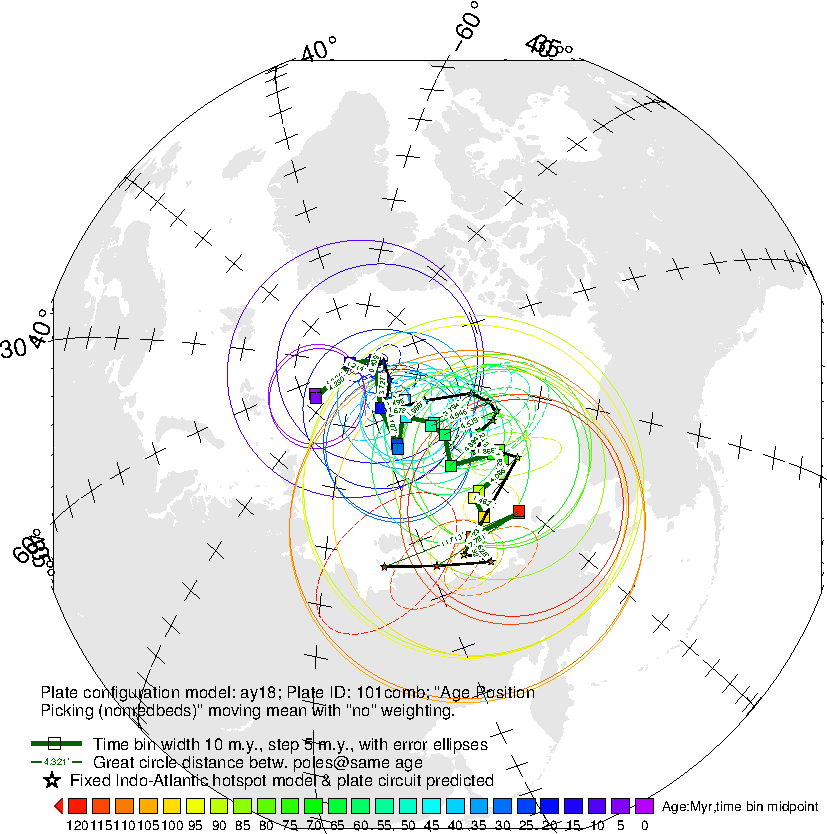
\includegraphics[width=\textwidth]{figures/ay18_101comb_10_5_11_0.pdf}
		\caption{North America (101): minimum 0.0053 (11, 0)}\label{fig-nac-105110}
	\end{subfigure}
	\begin{subfigure}{.42\textwidth} % width of right subfigure
		\includegraphics[width=\textwidth]{figures/ay18_101comb_10_5_16_3.pdf}
		\caption{North America (101): maximum 0.0921 (16, 3)}\label{fig-nac-105163}
	\end{subfigure}
	\vspace{.1em}
	\begin{subfigure}{.42\textwidth}
		\includegraphics[width=\textwidth]{figures/ay18_501comb_10_5_19_0.pdf}
		\caption{India (501): minimum 0.023 (19, 0)}\label{fig-ind-105190}
	\end{subfigure}
	\begin{subfigure}{.42\textwidth}
		\includegraphics[width=\textwidth]{figures/ay18_501comb_10_5_8_3.pdf}
		\caption{India (501): maximum 0.5137 (8, 3)}\label{fig-ind-10583}
	\end{subfigure}
	\vspace{.1em}
	\begin{subfigure}{.42\textwidth}
		\includegraphics[width=\textwidth]{figures/ay18_801comb_10_5_17_0.pdf}
		\caption{Australia (801): minimum 0.0037 (17, 0)}\label{fig-au-105170}
	\end{subfigure}
	\begin{subfigure}{.42\textwidth}
		\includegraphics[width=\textwidth]{figures/ay18_801comb_10_5_22_3.pdf}
		\caption{Australia (801): maximum 0.3954 (22, 3)}\label{fig-au-105223}
	\end{subfigure}
	\caption[Best and worst differences with test (10 Myr bin, 5 Myr
step)]{Path comparisons with best and worst difference values shown in
Fig.~\ref{fig-dif}.}\label{fig-difbw}
\end{figure*}

\begin{figure*}
	\centering
	\begin{subfigure}{1.01\textwidth}
		\includegraphics[width=\textwidth]{figures/f501d101.pdf}
		\caption{India (501) - North America (101)}\label{fig-i-n-dif}
	\end{subfigure}
	\vspace{1em}
	\begin{subfigure}{1.01\textwidth}
		\includegraphics[width=\textwidth]{figures/f801d101.pdf}
		\caption{Australia (801) - North America (101)}\label{fig-a-n-dif}
	\end{subfigure}
	\vspace{1em}
	\begin{subfigure}{1.01\textwidth}
		\includegraphics[width=\textwidth]{figures/f501d801.pdf}
		\caption{India (501) - Australia (801)}\label{fig-i-a-dif}
	\end{subfigure}
	\caption[Differences of differences with test of each plate's paleomagnetic
APWPs versus its FHM predicted APWP]{Differences between grids in
Fig.~\ref{fig-dif}. The absolute difference values less than
1.96-standard-deviation interval of the whole 168 values are labeled in green,
more than 1.96-standard-deviation interval labeled in red.}\label{fig-d-dif}
\end{figure*}

\begin{figure*}
	\centering
	\begin{subfigure}{1.01\textwidth}
		\includegraphics[width=\textwidth]{figures/101_120_0AMPvsAPP.pdf}
		\caption{North America: AMP: minimum 0.00796 (4, 0), maximum 0.0921 (16,
		3), mean 0.04515, median 0.04664; APP: minimum 0.0053 (11, 0), maximum
		0.05686 (5/7, 3), mean 0.02059, median 0.01594}\label{fig-na-difAMPvsAPP}
	\end{subfigure}
	\vspace{.1em}
	\begin{subfigure}{1.01\textwidth}
		\includegraphics[width=\textwidth]{figures/501_120_0AMPvsAPP.pdf}
		\caption{India: AMP: minimum 0.0292 (4, 3), maximum 0.5137 (8, 3), mean
		0.1668, median 0.1862; APP: minimum 0.023 (19, 0), maximum 0.1359 (3,
		4), mean 0.06798, median 0.0609}\label{fig-in-difAMPvsAPP}
	\end{subfigure}
	\vspace{.1em}
	\begin{subfigure}{1.01\textwidth}
		\includegraphics[width=\textwidth]{figures/801_120_0AMPvsAPP.pdf}
		\caption{Australia: AMP: minimum 0.0231 (4, 0), maximum 0.3954 (22,
		3), mean 0.1203, median 0.0598; APP: minimum 0.0037 (17, 0), maximum
		0.11035 (15, 3), mean 0.04225, median 0.02692}\label{fig-au-difAMPvsAPP}
	\end{subfigure}
	\caption[Differences with test of each plate's paleomagnetic APWPs versus
its FHM predicted APWP (AMP vs APP)]{Separated results from AMP and APP in
Fig.~\ref{fig-dif}. For each grid block (left: AMP; right: APP), the difference
values less than one-standard-deviation interval of the whole 84 values are
labeled in green, more than one-standard-deviation interval labeled in
red.}\label{fig-difAMPvsAPP}
\end{figure*}

\subparagraph{Measure 2: Only Space Tested}

According to the results (Fig.~\ref{fig-nant-dif}, Fig.~\ref{fig-indnt-dif} and
Fig.~\ref{fig-aunt-dif}), we can observe:
%
\begin{enumerate}
  \item the groups of picking-method-no 1, 19, 21 and 25 are the best, and 2
        and 14 the worst, for all the three continents.
\end{enumerate}

\begin{figure*}
	\centering
	\begin{subfigure}{1.01\textwidth}
		\includegraphics[width=\textwidth]{figures/101_120_0_.pdf}
		\caption{North America (101): minimum 0.2536 (1, 1), maximum 0.5104 (14, 4), mean 0.3837, median 0.3912}\label{fig-nant-dif}
	\end{subfigure}
	\vspace{.1em}
	\begin{subfigure}{1.01\textwidth}
		\includegraphics[width=\textwidth]{figures/501_120_0_.pdf}
		\caption{India (501): minimum 0.282 (6, 5), maximum 0.7637 (8, 3), mean 0.4667, median 0.4532}\label{fig-indnt-dif}
	\end{subfigure}
	\vspace{.1em}
	\begin{subfigure}{1.01\textwidth}
		\includegraphics[width=\textwidth]{figures/801_120_0_.pdf}
		\caption{Australia (801): minimum 0.2246 (11, 0), maximum 0.7554 (22, 3), mean 0.502, median 0.5142}\label{fig-aunt-dif}
	\end{subfigure}
	\caption[Differences without shape test of each plate's paleomagnetic APWPs
versus its FHM predicted APWP]{Difference values without shape test between each
continent's paleomagnetic APWPs and its predicted APWP from FHM and related
plate circuits. The paths are in 10 Myr bin and 5 Myr step. The difference
values less than one-standard-deviation interval of the whole 168 values are
labeled in green, more than one-standard-deviation interval labeled in red. See
the numbers of picked paleo-poles in Fig.~\ref{fig-dif}.}\label{fig-difnt}
\end{figure*}

\begin{figure*}
	\centering
	\begin{subfigure}{.42\textwidth}
		\includegraphics[width=\textwidth]{figures/ay18_101comb_10_5_1_1.pdf}
		\caption{North America (101): minimum 0.2536 (1, 1)}\label{fig-nant-10511}
	\end{subfigure}
	\begin{subfigure}{.42\textwidth}
		\includegraphics[width=\textwidth]{figures/ay18_101comb_10_5_14_4.pdf}
		\caption{North America (101): maximum 0.5104 (14, 4)}\label{fig-nant-105144}
	\end{subfigure}
	\vspace{.1em}
	\begin{subfigure}{.42\textwidth}
		\includegraphics[width=\textwidth]{figures/ay18_501comb_10_5_6_5.pdf}
		\caption{India (501): minimum 0.282 (6, 5)}\label{fig-indnt-10565}
	\end{subfigure}
	\begin{subfigure}{.42\textwidth}
		\includegraphics[width=\textwidth]{figures/ay18_501comb_10_5_8_3.pdf}
		\caption{India (501): maximum 0.7637 (8, 3), same as Fig.~\ref{fig-ind-10583}}\label{fig-indnt-10583}
	\end{subfigure}
	\vspace{.1em}
	\begin{subfigure}{.42\textwidth}
		\includegraphics[width=\textwidth]{figures/ay18_801comb_10_5_11_0.pdf}
		\caption{Australia (801): minimum 0.2246 (11, 0)}\label{fig-aunt-105110}
	\end{subfigure}
	\begin{subfigure}{.42\textwidth}
		\includegraphics[width=\textwidth]{figures/ay18_801comb_10_5_22_3.pdf}
		\caption{Australia (801): maximum 0.7554 (22, 3), same as Fig.~\ref{fig-au-105223}}\label{fig-aunt-105223}
	\end{subfigure}
	\caption[Best and worst differences without shape test (10 Myr bin, 5 Myr
step)]{Path comparisons with best and worst difference values shown in
Fig.~\ref{fig-difnt}.}\label{fig-difntbw}
\end{figure*}

\paragraph{20 Myr Binning and 10 Myr Stepping}

\subparagraph{Measure 1: Both Space and Shape Tested}

According to the results (Fig.~\ref{fig-dif2010}), we can observe:
%
\begin{enumerate}
  \item the groups of picking-method-no 19 is the best, and 16 the worst, for
        all the three continents.
\end{enumerate}

\begin{figure*}
	\centering
	\begin{subfigure}{1.01\textwidth}
		\includegraphics[width=\textwidth]{figures/101_20_10_120_0.pdf}
		\caption{North America (101): minimum 0.0115 (13, 0), maximum 0.0635 (16, 2), mean 0.0335, median 0.0285}\label{fig-nac-dif2010}
	\end{subfigure}
	\vspace{1em}
	\begin{subfigure}{1.01\textwidth}
		\includegraphics[width=\textwidth]{figures/501_20_10_120_0.pdf}
		\caption{India (501): minimum 0.0143 (6, 3), maximum 0.1543 (16, 3), mean 0.074, median 0.0755}\label{fig-ind-dif2010}
	\end{subfigure}
	\vspace{1em}
	\begin{subfigure}{1.01\textwidth}
		\includegraphics[width=\textwidth]{figures/801_20_10_120_0.pdf}
		\caption{Australia (801): minimum 0.0022 (11, 0), maximum 0.3265 (22, 3), mean 0.0686, median 0.0346}\label{fig-au-dif2010}
	\end{subfigure}
	\caption[Differences with test of each plate's paleomagnetic APWPs versus
its FHM predicted APWP]{Same as Fig.~\ref{fig-dif}. The only difference is here
the paths are in 20 Myr bin and 10 Myr step. The difference values less than
one-standard-deviation interval of the whole 168 values are labeled in green,
more than one-standard-deviation interval labeled in red. See the numbers
of picked paleo-poles in Fig.~\ref{fig-dif}.}\label{fig-dif2010}
\end{figure*}

\begin{figure*}
	\centering
	\begin{subfigure}{.43\textwidth}
		\includegraphics[width=\textwidth]{figures/ay18_101comb_20_10_13_0.pdf}
		\caption{North America (101): minimum 0.0115 (13, 0)}\label{fig-nac-2010130}
	\end{subfigure}
	\begin{subfigure}{.43\textwidth}
		\includegraphics[width=\textwidth]{figures/ay18_101comb_20_10_16_2.pdf}
		\caption{North America (101): maximum 0.0635 (16, 2)}\label{fig-nac-2010162}
	\end{subfigure}
	\vspace{.1em}
	\begin{subfigure}{.43\textwidth}
		\includegraphics[width=\textwidth]{figures/ay18_501comb_20_10_6_3.pdf}
		\caption{India (501): minimum 0.0143 (6, 3)}\label{fig-ind-201063}
	\end{subfigure}
	\begin{subfigure}{.43\textwidth}
		\includegraphics[width=\textwidth]{figures/ay18_501comb_20_10_16_3.pdf}
		\caption{India (501): maximum 0.1543 (16, 3)}\label{fig-ind-2010163}
	\end{subfigure}
	\vspace{.1em}
	\begin{subfigure}{.43\textwidth}
		\includegraphics[width=\textwidth]{figures/ay18_801comb_20_10_11_0.pdf}
		\caption{Australia (801): minimum 0.0022 (11, 0)}\label{fig-au-2010110}
	\end{subfigure}
	\begin{subfigure}{.43\textwidth}
		\includegraphics[width=\textwidth]{figures/ay18_801comb_20_10_22_3.pdf}
		\caption{Australia (801): maximum 0.3265 (22, 3)}\label{fig-au-2010223}
	\end{subfigure}
	\caption[Best and worst differences with test (20 Myr bin, 10 Myr
step)]{Path comparisons with best and worst difference values shown in
Fig.~\ref{fig-dif2010}.}\label{fig-dif2010bw}
\end{figure*}

\subparagraph{Measure 2: Only Space Tested}

According to the results (Fig.~\ref{fig-dif2010nt}), we can observe:
%
\begin{enumerate}
  \item the groups of picking-method-no 11, 13, 19 and 21 are the best, and 16
        the worst, for all the three continents.
\end{enumerate}

\begin{figure*}
	\centering
	\begin{subfigure}{1.01\textwidth}
		\includegraphics[width=\textwidth]{figures/101_20_10_120_0_.pdf}
		\caption{North America (101): minimum 0.2768 (19, 0), maximum 0.4683 (14, 5), mean 0.3773, median 0.3855}\label{fig-nant-dif2010}
	\end{subfigure}
	\vspace{.1em}
	\begin{subfigure}{1.01\textwidth}
		\includegraphics[width=\textwidth]{figures/501_20_10_120_0_.pdf}
		\caption{India (501): minimum 0.2676 (7, 3), maximum 0.5027 (23, 1; 27, 1), mean 0.3914, median 0.408}\label{fig-indnt-dif2010}
	\end{subfigure}
	\vspace{.1em}
	\begin{subfigure}{1.01\textwidth}
		\includegraphics[width=\textwidth]{figures/801_20_10_120_0_.pdf}
		\caption{Australia (801): minimum 0.1849 (11, 1), maximum 0.5772 (22, 2), mean 0.3882, median 0.3892}\label{fig-aunt-dif2010}
	\end{subfigure}
	\caption[Differences without shape test of each plate's paleomagnetic APWPs
versus its FHM predicted APWP]{Same as Fig.~\ref{fig-difnt}. The only difference
is here the paths are in 20 Myr bin and 10 Myr step. The difference values less
than one-standard-deviation interval of the whole 168 values are labeled in
green, more than one-standard-deviation interval labeled in red. See the numbers
of picked paleo-poles in Fig.~\ref{fig-dif}.}\label{fig-dif2010nt}
\end{figure*}

\begin{figure*}
	\centering
	\begin{subfigure}{.43\textwidth}
		\includegraphics[width=\textwidth]{figures/ay18_101comb_20_10_19_0.pdf}
		\caption{North America (101): minimum 0.2768 (19, 0)}\label{fig-nant-2010190}
	\end{subfigure}
	\begin{subfigure}{.43\textwidth}
		\includegraphics[width=\textwidth]{figures/ay18_101comb_20_10_14_5.pdf}
		\caption{North America (101): maximum 0.4683 (14, 5)}\label{fig-nant-2010145}
	\end{subfigure}
	\vspace{.1em}
	\begin{subfigure}{.43\textwidth}
		\includegraphics[width=\textwidth]{figures/ay18_501comb_20_10_7_3.pdf}
		\caption{India (501): minimum 0.2676 (7, 3)}\label{fig-indnt-201073}
	\end{subfigure}
	\begin{subfigure}{.43\textwidth}
		\includegraphics[width=\textwidth]{figures/ay18_501comb_20_10_23_1.pdf}
		\caption{India (501): maximum 0.5027 (23, 1; 27, 1)}\label{fig-indnt-2010231}
	\end{subfigure}
	\vspace{.1em}
	\begin{subfigure}{.43\textwidth}
		\includegraphics[width=\textwidth]{figures/ay18_801comb_20_10_11_1.pdf}
		\caption{Australia (801): minimum 0.1849 (11, 1)}\label{fig-aunt-2010111}
	\end{subfigure}
	\begin{subfigure}{.43\textwidth}
		\includegraphics[width=\textwidth]{figures/ay18_801comb_20_10_22_2.pdf}
		\caption{Australia (801): maximum 0.5772 (22, 2)}\label{fig-aunt-2010222}
	\end{subfigure}
	\caption[Best and worst differences without shape test (20 Myr bin, 10 Myr
step)]{Path comparisons with best and worst difference values shown in
Fig.~\ref{fig-dif2010nt}.}\label{fig-dif2010ntbw}
\end{figure*}

\subsubsection{When MHM and Global Plate Tectonic Circuits Predicted APWP as
Reference}

Then, we focus on analysing the results with MHM and global plate circuits
predicted APWP (Fig.~\ref{fig-mhsPred}, Fig.~\ref{fig-mhsPred501},
Fig.~\ref{fig-mhsPred801}) as the reference path.

\begin{figure*}
	\centering
	\begin{subfigure}{1.01\textwidth}
		\includegraphics[width=\textwidth]{figures/101_120_0m.pdf}
		\caption{North America (101): minimum 0.00077 (4, 0), maximum 0.0926 (16, 5), mean 0.0361, median 0.0325}\label{fig-nac-difm}
	\end{subfigure}
	\vspace{1em}
	\begin{subfigure}{1.01\textwidth}
		\includegraphics[width=\textwidth]{figures/501_120_0m.pdf}
		\caption{India (501): minimum 0.0228 (4, 3), maximum 0.5188 (8, 3), mean 0.113, median 0.0746}\label{fig-ind-difm}
	\end{subfigure}
	\vspace{1em}
	\begin{subfigure}{1.01\textwidth}
		\includegraphics[width=\textwidth]{figures/801_120_0m.pdf}
		\caption{Australia (801): minimum 0.0024 (17, 5), maximum 0.3662 (22, 3), mean 0.0744, median 0.0374}\label{fig-au-difm}
	\end{subfigure}
	\caption[Differences with test of each plate's paleomagnetic APWPs versus
its MHM predicted APWP]{Same as Fig.~\ref{fig-dif} except that the reference
path is predicted from MHM here. See the numbers of picked paleo-poles in
Fig.~\ref{fig-dif}.}\label{fig-difm}
\end{figure*}

\begin{figure*}
	\centering
	\begin{subfigure}{.42\textwidth}
		\includegraphics[width=\textwidth]{figures/ay18_101comb_10_5_4_0m.pdf}
		\caption{North America (101): minimum 0.00077 (4, 0)}\label{fig-nac-10540m}
	\end{subfigure}
	\begin{subfigure}{.42\textwidth}
		\includegraphics[width=\textwidth]{figures/ay18_101comb_10_5_16_5m.pdf}
		\caption{North America (101): maximum 0.0926 (16, 5)}\label{fig-nac-105165m}
	\end{subfigure}
	\vspace{.1em}
	\begin{subfigure}{.42\textwidth}
		\includegraphics[width=\textwidth]{figures/ay18_501comb_10_5_4_3m.pdf}
		\caption{India (501): minimum 0.0228 (4, 3)}\label{fig-ind-10543m}
	\end{subfigure}
	\begin{subfigure}{.42\textwidth}
		\includegraphics[width=\textwidth]{figures/ay18_501comb_10_5_8_3m.pdf}
		\caption{India (501): maximum 0.5188 (8, 3)}\label{fig-ind-10583m}
	\end{subfigure}
	\vspace{.1em}
	\begin{subfigure}{.42\textwidth}
		\includegraphics[width=\textwidth]{figures/ay18_801comb_10_5_17_5m.pdf}
		\caption{Australia (801): minimum 0.0024 (17, 5)}\label{fig-au-105175m}
	\end{subfigure}
	\begin{subfigure}{.42\textwidth}
		\includegraphics[width=\textwidth]{figures/ay18_801comb_10_5_22_3m.pdf}
		\caption{Australia (801): maximum 0.3662 (22, 3)}\label{fig-au-105223m}
	\end{subfigure}
	\caption[Best and worst differences with test (10 Myr bin, 5 Myr
step)]{Path comparisons with best and worst difference values shown in
Fig.~\ref{fig-difm}.}\label{fig-difbwm}
\end{figure*}

\paragraph{10 Myr Binning and 5 Myr Stepping}

\subparagraph{Measure 1: Both Space and Shape Tested}

According to the results (Fig.~\ref{fig-nac-difm}, Fig.~\ref{fig-ind-difm} and
Fig.~\ref{fig-au-difm}), we can observe:
%
\begin{enumerate}
  \item there is no best picking method, whereas no. 16 is the worst, for all
		the three continents.
\end{enumerate}

\begin{figure*}
	\centering
	\begin{subfigure}{1.01\textwidth}
		\includegraphics[width=\textwidth]{figures/101_120_0_m.pdf}
		\caption{North America (101): minimum 0.2147 (11, 0), maximum 0.5183 (16, 3), mean 0.3702, median 0.3642}\label{fig-nant-difm}
	\end{subfigure}
	\vspace{.1em}
	\begin{subfigure}{1.01\textwidth}
		\includegraphics[width=\textwidth]{figures/501_120_0_m.pdf}
		\caption{India (501): minimum 0.2961 (26, 3), maximum 0.7779 (8, 3), mean 0.4578, median 0.4306}\label{fig-indnt-difm}
	\end{subfigure}
	\vspace{.1em}
	\begin{subfigure}{1.01\textwidth}
		\includegraphics[width=\textwidth]{figures/801_120_0_m.pdf}
		\caption{Australia (801): minimum 0.2008 (11, 1), maximum 0.7136 (26, 4), mean 0.46, median 0.4726}\label{fig-aunt-difm}
	\end{subfigure}
	\caption[Differences without shape test of each plate's paleomagnetic APWPs
versus its MHM predicted APWP]{Same as Fig.~\ref{fig-difnt} except that the
reference path is predicted from MHM here. See the numbers of picked paleo-poles
in Fig.~\ref{fig-dif}.}\label{fig-difntm}
\end{figure*}

\begin{figure*}
	\centering
	\begin{subfigure}{.42\textwidth}
		\includegraphics[width=\textwidth]{figures/ay18_101comb_10_5_11_0m.pdf}
		\caption{North America (101): minimum 0.2147 (11, 0)}\label{fig-nant-105110m}
	\end{subfigure}
	\begin{subfigure}{.42\textwidth}
		\includegraphics[width=\textwidth]{figures/ay18_101comb_10_5_16_3m.pdf}
		\caption{North America (101): maximum 0.5183 (16, 3)}\label{fig-nant-105163m}
	\end{subfigure}
	\vspace{.1em}
	\begin{subfigure}{.42\textwidth}
		\includegraphics[width=\textwidth]{figures/ay18_501comb_10_5_26_3m.pdf}
		\caption{India (501): minimum 0.2961 (26, 3)}\label{fig-indnt-105263m}
	\end{subfigure}
	\begin{subfigure}{.42\textwidth}
		\includegraphics[width=\textwidth]{figures/ay18_501comb_10_5_8_3m.pdf}
		\caption{India (501): maximum 0.7779 (8, 3), same as Fig.~\ref{fig-ind-10583m}}\label{fig-indnt-10583m}
	\end{subfigure}
	\vspace{.1em}
	\begin{subfigure}{.42\textwidth}
		\includegraphics[width=\textwidth]{figures/ay18_801comb_10_5_11_1m.pdf}
		\caption{Australia (801): minimum 0.2008 (11, 1)}\label{fig-aunt-105111m}
	\end{subfigure}
	\begin{subfigure}{.42\textwidth}
		\includegraphics[width=\textwidth]{figures/ay18_801comb_10_5_26_4m.pdf}
		\caption{Australia (801): maximum 0.7136 (26, 4)}\label{fig-aunt-105264m}
	\end{subfigure}
	\caption[Best and worst differences without shape test (10 Myr bin, 5 Myr
step)]{Path comparisons with best and worst difference values shown in
Fig.~\ref{fig-difntm}.}\label{fig-difntbwm}
\end{figure*}

\subparagraph{Measure 2: Only Space Tested}

According to the results (Fig.~\ref{fig-nant-difm}, Fig.~\ref{fig-indnt-difm}
and Fig.~\ref{fig-aunt-difm}), we can observe:
%
\begin{enumerate}
  \item the groups of picking-method-no 1, 19 and 21 are the best, and 8, 10
        and 14 the worst, for all the three continents.
\end{enumerate}

\begin{figure*}
	\centering
	\begin{subfigure}{1.01\textwidth}
		\includegraphics[width=\textwidth]{figures/101_20_10_120_0m.pdf}
		\caption{North America (101): minimum 0.0058 (15, 5), maximum 0.1041 (8, 4), mean 0.0437, median 0.0267}\label{fig-nac-dif2010m}
	\end{subfigure}
	\vspace{1em}
	\begin{subfigure}{1.01\textwidth}
		\includegraphics[width=\textwidth]{figures/501_20_10_120_0m.pdf}
		\caption{India (501): minimum 0.0177 (6, 3), maximum 0.162 (16, 3), mean 0.0759, median 0.0621}\label{fig-ind-dif2010m}
	\end{subfigure}
	\vspace{1em}
	\begin{subfigure}{1.01\textwidth}
		\includegraphics[width=\textwidth]{figures/801_20_10_120_0m.pdf}
		\caption{Australia (801): minimum 0.0047 (23, 4), maximum 0.3158 (26, 3), mean 0.0638, median 0.0307}\label{fig-au-dif2010m}
	\end{subfigure}
	\caption[Differences with test of each plate's paleomagnetic APWPs versus
its MHM predicted APWP]{Same as Fig.~\ref{fig-dif2010} except that the reference
path is predicted from MHM here. See the numbers of picked paleo-poles in
Fig.~\ref{fig-dif}.}\label{fig-dif2010m}
\end{figure*}

\begin{figure*}
	\centering
	\begin{subfigure}{.43\textwidth}
		\includegraphics[width=\textwidth]{figures/ay18_101comb_20_10_15_5m.pdf}
		\caption{North America (101): minimum 0.0058 (15, 5)}\label{fig-nac-2010155m}
	\end{subfigure}
	\begin{subfigure}{.43\textwidth}
		\includegraphics[width=\textwidth]{figures/ay18_101comb_20_10_8_4m.pdf}
		\caption{North America (101): maximum 0.1041 (8, 4)}\label{fig-nac-201084m}
	\end{subfigure}
	\vspace{.1em}
	\begin{subfigure}{.43\textwidth}
		\includegraphics[width=\textwidth]{figures/ay18_501comb_20_10_6_3m.pdf}
		\caption{India (501): minimum 0.0177 (6, 3)}\label{fig-ind-201063m}
	\end{subfigure}
	\begin{subfigure}{.43\textwidth}
		\includegraphics[width=\textwidth]{figures/ay18_501comb_20_10_16_3m.pdf}
		\caption{India (501): maximum 0.162 (16, 3)}\label{fig-ind-2010163m}
	\end{subfigure}
	\vspace{.1em}
	\begin{subfigure}{.43\textwidth}
		\includegraphics[width=\textwidth]{figures/ay18_801comb_20_10_23_4m.pdf}
		\caption{Australia (801): minimum 0.0047 (23, 4)}\label{fig-au-2010234m}
	\end{subfigure}
	\begin{subfigure}{.43\textwidth}
		\includegraphics[width=\textwidth]{figures/ay18_801comb_20_10_26_3m.pdf}
		\caption{Australia (801): maximum 0.3158 (26, 3)}\label{fig-au-2010263m}
	\end{subfigure}
	\caption[Best and worst differences with test (20 Myr bin, 10 Myr
step)]{Path comparisons with best and worst difference values shown in
Fig.~\ref{fig-dif2010m}.}\label{fig-dif2010bwm}
\end{figure*}

\paragraph{20 Myr Binning and 10 Myr Stepping}

\subparagraph{Measure 1: Both Space and Shape Tested}

According to the results (Fig.~\ref{fig-dif2010m}), we can observe:
%
\begin{enumerate}
  \item there is no best picking method, whereas no. 16 is the worst, for all
		the three continents.
\end{enumerate}

\begin{figure*}
	\centering
	\begin{subfigure}{1.01\textwidth}
		\includegraphics[width=\textwidth]{figures/101_20_10_120_0_m.pdf}
		\caption{North America (101): minimum 0.1923 (4, 0), maximum 0.4794 (16, 2), mean 0.3384, median 0.3318}\label{fig-nant-dif2010m}
	\end{subfigure}
	\vspace{.1em}
	\begin{subfigure}{1.01\textwidth}
		\includegraphics[width=\textwidth]{figures/501_20_10_120_0_m.pdf}
		\caption{India (501): minimum 0.2462 (6, 0), maximum 0.5417 (8, 3), mean 0.3858, median 0.3659}\label{fig-indnt-dif2010m}
	\end{subfigure}
	\vspace{.1em}
	\begin{subfigure}{1.01\textwidth}
		\includegraphics[width=\textwidth]{figures/801_20_10_120_0_m.pdf}
		\caption{Australia (801): minimum 0.2091 (5, 5), maximum 0.5777 (14, 0), mean 0.3694, median 0.3676}\label{fig-aunt-dif2010m}
	\end{subfigure}
	\caption[Differences without shape test of each plate's paleomagnetic APWPs
versus its MHM predicted APWP]{Same as Fig.~\ref{fig-dif2010nt} except that the
reference path is predicted from MHM here. See the numbers of picked paleo-poles
in Fig.~\ref{fig-dif}.}\label{fig-dif2010ntm}
\end{figure*}

\begin{figure*}
	\centering
	\begin{subfigure}{.43\textwidth}
		\includegraphics[width=\textwidth]{figures/ay18_101comb_20_10_4_0m.pdf}
		\caption{North America (101): minimum 0.1923 (4, 0)}\label{fig-nant-201040m}
	\end{subfigure}
	\begin{subfigure}{.43\textwidth}
		\includegraphics[width=\textwidth]{figures/ay18_101comb_20_10_16_2m.pdf}
		\caption{North America (101): maximum 0.4794 (16, 2)}\label{fig-nant-2010162m}
	\end{subfigure}
	\vspace{.1em}
	\begin{subfigure}{.43\textwidth}
		\includegraphics[width=\textwidth]{figures/ay18_501comb_20_10_6_0m.pdf}
		\caption{India (501): minimum 0.2462 (6, 0)}\label{fig-indnt-201060m}
	\end{subfigure}
	\begin{subfigure}{.43\textwidth}
		\includegraphics[width=\textwidth]{figures/ay18_501comb_20_10_8_3m.pdf}
		\caption{India (501): maximum 0.5417 (8, 3)}\label{fig-indnt-201083m}
	\end{subfigure}
	\vspace{.1em}
	\begin{subfigure}{.43\textwidth}
		\includegraphics[width=\textwidth]{figures/ay18_801comb_20_10_5_5m.pdf}
		\caption{Australia (801): minimum 0.2091 (5, 5)}\label{fig-aunt-201055m}
	\end{subfigure}
	\begin{subfigure}{.43\textwidth}
		\includegraphics[width=\textwidth]{figures/ay18_801comb_20_10_14_0m.pdf}
		\caption{Australia (801): maximum 0.5777 (14, 0)}\label{fig-aunt-2010140m}
	\end{subfigure}
	\caption[Best and worst differences without shape test (20 Myr bin, 10 Myr
step)]{Path comparisons with best and worst difference values shown in
Fig.~\ref{fig-dif2010ntm}.}\label{fig-dif2010ntbwm}
\end{figure*}

\subparagraph{Measure 2: Only Space Tested}

According to the results (Fig.~\ref{fig-dif2010ntm}), we can observe:
%
\begin{enumerate}
  \item the groups of picking-method-no 15 and 19 are the best, and 8 the worst,
		for all the three continents.
\end{enumerate}

\subsubsection{Summary of Results}

\begin{table*}
\centering
\caption{Performance statistics of all the picking and weighting methods.}
\label{tab-bw}
\resizebox{\textwidth}{!}{%
\begin{tabular}{l|l|l|l|l|l|l|l|l|l|l|l|l|l}
\multicolumn{2}{l|}{\multirow{2}{*}{Grid}} & \multicolumn{2}{l|}{Best No.} &
  \multicolumn{2}{l|}{Worst No.} & \multirow{2}{*}{\parbox{1.8cm}{Proportion of
  APP Better Than AMP}} & \multicolumn{6}{l|}{\multirow{2}{*}{\parbox{5cm}{For
  All 28 Picking Methods, Count of Occurrences of Each Weighting No. Being
  Best}}} & \multirow{2}{*}{\parbox{2.6cm}{Picking 14/15 (Studies After 1983)
  Better Than 16/17 (Older)}} \\ \\ \cline{3-6} \cline{8-13}
\multicolumn{2}{l|}{} & Picking & Weighting & Picking & Weighting &  & 0 & 1 &
  2 & 3 & 4 & 5 &  \\ \hline
\multirow{12}{*}{FHM}
& Fig.~\ref{fig-nac-dif} & \multirow{2}{*}{\parbox{2cm}{1, 4, 5, 7, 11, 13, 15,
  \textbf{19}, \textbf{21}, 25}} & \multirow{2}{*}{\parbox{1cm}{0, 1, 5}} &
  \multirow{2}{*}{\parbox{2cm}{2, 5, 7, 8, 14, \textbf{16}, 17, 18, 22, 26}} &
  \multirow{2}{*}{\parbox{1cm}{0, 1, 2, 3, 4, 5}} & 27/28 & \textbf{15} & 4 & 2 & 3 & 1
  & 4 & Y/Y \\ \\ \cline{2-14}
& Fig.~\ref{fig-nant-dif} & \multirow{2}{*}{\parbox{2cm}{1, 11, 13, 15,
  \textbf{19}, \textbf{21}, 25}} & \multirow{2}{*}{\parbox{1cm}{0, 1, 2, 4, 5}} &
  \multirow{2}{*}{\parbox{2.4cm}{0, 2, 3, 8, 10, 12, 14, \textbf{16}, 17, 18, 20, 24}} &
  \multirow{2}{*}{\parbox{1cm}{0, 1, 2, 3, 4, 5}} & 71/84 & 9 & \textbf{13} & 0 & 1 & 1
  & 4 & N/Y \\ \\ \cline{2-14}
& Fig.~\ref{fig-ind-dif} & \multirow{2}{*}{\parbox{2cm}{4, 5, 6, 7, 9,
  \textbf{19}, \textbf{21}}} & \multirow{2}{*}{\parbox{1cm}{0, 1, 2, 3, 4, 5}} &
  \multirow{2}{*}{\parbox{2.4cm}{0, 2, 8, 10, 12, \textbf{16}, 18, 20, 24}} &
  \multirow{2}{*}{\parbox{1cm}{0, 1, 2, 3, 4, 5}} & 11/14 & \textbf{17} & 1 & 2 & 7 & 1
  & 0 & Y/Y \\ \\ \cline{2-14}
& Fig.~\ref{fig-indnt-dif} & \multirow{2}{*}{\parbox{2cm}{1, 4, 6, 9, 17,
  \textbf{19}, \textbf{21}, 25, 26}} & \multirow{2}{*}{\parbox{1cm}{0, 1, 2, 3, 4, 5}} &
  \multirow{2}{*}{\parbox{2.4cm}{0, 2, 8, 10, 12, 14, \textbf{16}, 18, 24}} &
  \multirow{2}{*}{\parbox{1cm}{0, 1, 2, 3, 4, 5}} & 5/7 & \textbf{13} & 1 & 4 & 5 & 0 &
  5& Y(4y2n)/Y(4y2n) \\ \\ \cline{2-14}
& Fig.~\ref{fig-au-dif} & \multirow{2}{*}{\parbox{2cm}{1, 11, 13, 17,
  \textbf{19}, \textbf{21}, 25}} & \multirow{2}{*}{\parbox{1cm}{0, 1, 3, 5}} &
  \multirow{2}{*}{\parbox{2.4cm}{2, 6, 14, \textbf{16}, 22, 26}} &
  \multirow{2}{*}{\parbox{1cm}{0, 1, 2, 3, 4, 5}} & 27/28 & \textbf{11} & 4 & 1 & 8 & 3
  & 1 & N/N \\ \\ \cline{2-14}
& Fig.~\ref{fig-aunt-dif} & \multirow{2}{*}{\parbox{2cm}{1, 7, 11, 13, 17,
  \textbf{19}, \textbf{21}, 25}} & \multirow{2}{*}{\parbox{1cm}{0, 1, 3, 5}} &
  \multirow{2}{*}{\parbox{2.4cm}{2, 6, 14, 22, 26}} &
  \multirow{2}{*}{\parbox{1cm}{0, 1, 2, 3, 4, 5}} & 1 & \textbf{9} & 6 & 2 & 7 & 2 & 2 &
  N/N \\ \\ \cline{2-14}
& Fig.~\ref{fig-nac-dif2010} & \multirow{2}{*}{\parbox{2cm}{1, 4, 5, 7, 11, 13,
  15, \textbf{19}, \textbf{21}, 25}} & \multirow{2}{*}{\parbox{1cm}{0, 1, 3, 5}} &
  \multirow{2}{*}{\parbox{2.4cm}{2, 6, 14, 22, 26}} &
  \multirow{2}{*}{\parbox{1cm}{0, 1, 2, 3, 4, 5}} & 3/4 & \textbf{18} & 6 & 0 & 2 & 4 &
  3 & N(5n1y)/Y \\ \\ \cline{2-14}
& Fig.~\ref{fig-nant-dif2010} & \multirow{2}{*}{\parbox{2cm}{1, 4, 5, 6, 7, 9,
  11, 13, 15, \textbf{19}, \textbf{21}, 25}} & \multirow{2}{*}{\parbox{1cm}{0, 1, 3, 5}} &
  \multirow{2}{*}{\parbox{2.4cm}{0, 3, 8, 10, 11, 12, 14, \textbf{16}, 17, 18, 20, 24}}
  & \multirow{2}{*}{\parbox{1cm}{0, 1, 2, 3, 4, 5}} & 17/21 & \textbf{15} & 6 & 0 & 2 &
  3& 2 & N/Y \\ \\ \cline{2-14}
& Fig.~\ref{fig-ind-dif2010} & \multirow{2}{*}{\parbox{2cm}{4, 5, 6, 7,
  \textbf{19}}} & \multirow{2}{*}{\parbox{1cm}{0, 1, 2, 3, 4, 5}} &
  \multirow{2}{*}{\parbox{2.4cm}{0, 2, 10, 12, \textbf{16}, 18, 20, 23, 24, 27}} &
  \multirow{2}{*}{\parbox{1cm}{0, 1, 2, 3, 4, 5}} & 59/84 & \textbf{12} & 6 & 0 & 9 & 0
  & 1 & Y/Y(4y2n) \\ \\ \cline{2-14}
& Fig.~\ref{fig-indnt-dif2010} & \multirow{2}{*}{\parbox{2cm}{4, 5, 6, 7, 9, 11,
  13, \textbf{19}, \textbf{21}}} & \multirow{2}{*}{\parbox{1cm}{0, 1, 2, 3, 4, 5}} &
  \multirow{2}{*}{\parbox{2cm}{0, 2, 8, 10, 12, \textbf{16}, 23, 24,
  27}} & \multirow{2}{*}{\parbox{1cm}{0, 1, 2, 3, 4, 5}} & 11/14 & \textbf{9} & 3 & 2 &
  8 & 3 & 3 & Y(4y2n)/N(5n1y) \\ \\ \cline{2-14}
& Fig.~\ref{fig-au-dif2010} & \multirow{2}{*}{\parbox{2cm}{1, 11, 13, 17,
\textbf{19}, \textbf{21}, 25}} & \multirow{2}{*}{\parbox{1cm}{0, 1, 3, 4, 5}} &
  \multirow{2}{*}{\parbox{2cm}{2, 14, \textbf{16}, 22, 26}} &
  \multirow{2}{*}{\parbox{1cm}{0, 1, 2, 3, 4, 5}} & 41/42 & 7 & 9 & 0 & \textbf{11} & 1
  & 2 & N/N(4n2y) \\ \\ \cline{2-14}
& Fig.~\ref{fig-aunt-dif2010} & \multirow{2}{*}{\parbox{2cm}{1, 11, 13, 15, 17,
  \textbf{19}, \textbf{21}, 25}} & \multirow{2}{*}{\parbox{1cm}{0, 1, 3, 5}} &
  \multirow{2}{*}{\parbox{2cm}{2, 4, 5, 14, \textbf{16}, 22, 26}} &
  \multirow{2}{*}{\parbox{1cm}{0, 1, 2, 3, 4, 5}} & 41/42 & 6 & 8 & 0 & \textbf{10} & 1
  & 3 & N/N(4n2y) \\ \\ \hline
\multirow{12}{*}{MHM}
& Fig.~\ref{fig-nac-difm} & \multirow{2}{*}{\parbox{2cm}{1, 4, 5, 7, 11, 13, 15,
  \textbf{21}, 25}} & \multirow{2}{*}{\parbox{1cm}{0, 1, 2, 3, 4, 5}} &
  \multirow{2}{*}{\parbox{2.2cm}{0, 8, 10, 12, 14, \textbf{16}, 17, 18, 20, 22, 24}} &
  \multirow{2}{*}{\parbox{1cm}{0, 1, 2, 3, 4, 5}} & 11/12 & \textbf{14} & 6 & 1 & 1 & 2
  & 4 & Y/Y \\ \\ \cline{2-14}
& Fig.~\ref{fig-nant-difm} & \multirow{2}{*}{\parbox{2cm}{1, 5, 7, 11, 13, 15,
  \textbf{19}, \textbf{21}, 23, 25, 27}} &
  \multirow{2}{*}{\parbox{1cm}{0, 1, 3, 5}} &
  \multirow{2}{*}{\parbox{2.4cm}{0, 8, 10, 12, 14, \textbf{16}, 17, 18, 24}} &
  \multirow{2}{*}{\parbox{1cm}{0, 1, 2, 3, 4, 5}} & 27/28 & 6 & \textbf{12} & 0 & 2 & 0
  & 8 & Y/Y \\ \\ \cline{2-14}
& Fig.~\ref{fig-ind-difm} & \multirow{2}{*}{\parbox{2cm}{4, 5, 6, 7, \textbf{19}, 22, 26}} &
  \multirow{2}{*}{\parbox{1cm}{0, 1, 2, 3, 4, 5}} &
  \multirow{2}{*}{\parbox{2.4cm}{0, 2, 8, 10, 12, \textbf{16}, 18, 20, 24}} &
  \multirow{2}{*}{\parbox{1cm}{0, 1, 2, 3, 4, 5}} & 11/14 & \textbf{12} & 3 & 0 & 9 & 1
  & 3 & Y/Y \\ \\ \cline{2-14}
& Fig.~\ref{fig-indnt-difm} & \multirow{2}{*}{\parbox{2cm}{1, 4, 6, 15, 17,
  \textbf{19}, \textbf{21}, 22, 26}} & \multirow{2}{*}{\parbox{1cm}{0, 1, 2, 3, 4, 5}} &
  \multirow{2}{*}{\parbox{2.4cm}{0, 2, 8, 10, 12, 14, \textbf{16}, 24}} &
  \multirow{2}{*}{\parbox{1cm}{0, 1, 2, 3, 4, 5}} & 61/84 & 0 & 1 & 7 & 6 & 3 &
  \textbf{11} & Y/Y(4y2n) \\ \\ \cline{2-14}
& Fig.~\ref{fig-au-difm} & \multirow{2}{*}{\parbox{2cm}{1, 11, 13, 17,
  \textbf{19}, \textbf{21}, 25}} & \multirow{2}{*}{\parbox{1cm}{0, 1, 3, 5}} &
  \multirow{2}{*}{\parbox{2.4cm}{2, 14, \textbf{16}, 22, 26}} &
  \multirow{2}{*}{\parbox{1cm}{0, 1, 2, 3, 4, 5}} & 20/21 & 8 & 5 & 1 & \textbf{9} & 4
  & 1 & N/N \\ \\ \cline{2-14}
& Fig.~\ref{fig-aunt-difm} & \multirow{2}{*}{\parbox{2cm}{1, 11, 13, 17,
  \textbf{19}, \textbf{21}, 25}} & \multirow{2}{*}{\parbox{1cm}{0, 1, 3, 5}} &
  \multirow{2}{*}{\parbox{2.4cm}{2, 6, 8, 10, 14, 18, 22, 26}} &
  \multirow{2}{*}{\parbox{1cm}{0, 1, 2, 3, 4, 5}} & 1 & 8 & 3 & 0 & \textbf{11} & 1 & 5 &
  N/N \\ \\ \cline{2-14}
& Fig.~\ref{fig-nac-dif2010m} & \multirow{2}{*}{\parbox{2cm}{4, 5, 7, 11,
  15, 22, 26}} & \multirow{2}{*}{\parbox{1cm}{0, 1, 2, 3, 4, 5}} &
  \multirow{2}{*}{\parbox{2.4cm}{0, 8, 10, 12, 14, \textbf{16}, 18, 20, 24}} &
  \multirow{2}{*}{\parbox{1cm}{0, 1, 2, 3, 4, 5}} & 3/4 & \textbf{15} & 6 & 1 & 0 & 1 &
  5 & N(5n1y)/Y \\ \\ \cline{2-14}
& Fig.~\ref{fig-nant-dif2010m} & \multirow{2}{*}{\parbox{2cm}{1, 4, 5, 7,
  11, 13, 15, \textbf{19}, \textbf{21}, 25}} & \multirow{2}{*}{\parbox{1cm}{0, 1, 3, 4, 5}} &
  \multirow{2}{*}{\parbox{2.4cm}{0, 8, 10, 12, 14, \textbf{16}, 18, 20, 24}} &
  \multirow{2}{*}{\parbox{1cm}{0, 1, 2, 3, 4, 5}} & 6/7 & \textbf{8} & 6 & 2 & 6 &
  3 & 3 & Y(5y1n)/Y(5y1n) \\ \\ \cline{2-14}
& Fig.~\ref{fig-ind-dif2010m} & \multirow{2}{*}{\parbox{2cm}{4, 5, 6, 7,
  \textbf{19}}} & \multirow{2}{*}{\parbox{1cm}{0, 1, 2, 3, 4, 5}} &
  \multirow{2}{*}{\parbox{2.4cm}{0, 2, 10, 12, \textbf{16}, 18, 23, 24, 27}} &
  \multirow{2}{*}{\parbox{1cm}{0, 1, 2, 3, 4, 5}} & 29/42 & \textbf{8} & \textbf{8} & 2 & 5 & 3
  & 2 & Y/N(5n1y) \\ \\ \cline{2-14}
& Fig.~\ref{fig-indnt-dif2010m} & \multirow{2}{*}{\parbox{2cm}{6, 9, 15,
  17, \textbf{19}, 22, 23, 26, 27}} & \multirow{2}{*}{\parbox{1cm}{0, 1, 2, 3, 4, 5}} &
  \multirow{2}{*}{\parbox{2cm}{0, 2, 3, 8, 10, 12, \textbf{16}, 18, 24}} &
  \multirow{2}{*}{\parbox{1cm}{1, 2, 3, 4, 5}} & 61/84 & 5 & 4 & 3 &
  5 & 3 & \textbf{8} & Y/N(5n1y) \\ \\ \cline{2-14}
& Fig.~\ref{fig-au-dif2010m} & \multirow{2}{*}{\parbox{2cm}{1, 11, 13, 15, 17,
  \textbf{19}, \textbf{21}, 23, 25, 27}} & \multirow{2}{*}{\parbox{1cm}{0, 1, 2, 3, 4, 5}} &
  \multirow{2}{*}{\parbox{2cm}{2, 14, \textbf{16}, 22, 26}} &
  \multirow{2}{*}{\parbox{1cm}{0, 1, 2, 3, 4, 5}} & 41/42 & \textbf{9} & 5 & 0 & 8 & 5
  & 1 & N/Y(4y2n) \\ \\ \cline{2-14}
& Fig.~\ref{fig-aunt-dif2010m} & \multirow{2}{*}{\parbox{2cm}{1, 5, 7, 11, 13, 15,
  \textbf{19}, \textbf{21}, 23, 25}} & \multirow{2}{*}{\parbox{1cm}{0, 1, 3, 4, 5}} &
  \multirow{2}{*}{\parbox{2cm}{2, 6, 8, 14, 20, 22, 26}} &
  \multirow{2}{*}{\parbox{1cm}{0, 1, 2, 3, 4, 5}} & 1 & 7 & 4 & 0 & \textbf{12} & 4
  & 1 & N/Y(4y2n)
\end{tabular}%
}
\end{table*}

According to all the above results (Fig.~\ref{fig-dif}, Fig.~\ref{fig-difnt},
Fig.~\ref{fig-dif2010}, Fig.~\ref{fig-dif2010nt}), we can observe:
%
\begin{enumerate}
  \item generally the APP methods (adding data to a time window with overlapping
        age selection criterion) produce better similarities than the AMP
        methods (Table.~\ref{tab-bw}).
  \item the self-explanatory topography of bands indicates that the picking
        methods (Table.~\ref{tab-pick}) influence the similarity more than the
        weighting methods (Table.~\ref{tab-weit}) do.
  \item filtering (picking no 2\textendash7, 10, 11, and 14\textendash27) and
        correcting (picking no 8, 9, 12 and 13) has limited effectiveness.
  \item weighting is not always making similarities better. In fact, for quite
        many of the methods, no weighting is the best performer
		(Table.~\ref{tab-bw}).
  \item the picking method no 19 is always the best when the FHM predicted APWP
		is the reference.
  \item the weighting method no 0, 1 and 5 are generally producing better
        similarity than 2, 3 and 4.
  \item North America (101) owns better similarity results than Australia (801)
        and India (501), because its worst and mean composite differences are
		always less than the other two continents'.
  \item for both North America (101) and India (501), more recent studies
        generally give better results than (or results close to) older studies.
		However, this is not true for Australia (801) (Fig.~\ref{fig-au-dif} and
		Fig.~\ref{fig-aunt-dif}).
\end{enumerate}

\subsection{Discussions}

The following discussions will be in Q\&A style.

\subsubsection{Question: Why the APP methods generally produce better
similarities than AMP methods do?}

Paleomagnetic (Mean) A95 represents precision (how well constrained calculated
poles are), and (mean) coeval poles' GCD represents accuracy (how close
calculated poles are to the reference path; Fig.~\ref{fig-A95GCD105F} and
Fig.~\ref{fig-A95SGCD105F}). Compared with AMP, APP usually improves both and
generates paths with higher accuracy and also higher precision (generally
increasing N).

\begin{figure}
\captionsetup[subfigure]{singlelinecheck=off,justification=raggedright,aboveskip=-6pt,belowskip=-6pt}
\centering
  \begin{subfigure}[htbp]{.49\textwidth}
	\caption{}\includegraphics[width=\textwidth]{figures/a95gcd_10_5F.pdf}\label{fig-A95GCD105F}
  \end{subfigure}
  \begin{subfigure}[htbp]{.49\textwidth}
	\caption{}\includegraphics[width=\textwidth]{figures/a95Sgcd_10_5F.pdf}\label{fig-A95SGCD105F}
  \end{subfigure}
  \begin{subfigure}[htbp]{.49\textwidth}
	\caption{}\includegraphics[width=\textwidth]{figures/a95mSad10_5F.pdf}\label{fig-A95mSad105F}
  \end{subfigure}
  \begin{subfigure}[htbp]{.49\textwidth}
	\caption{}\includegraphics[width=\textwidth]{figures/a95mSld10_5F.pdf}\label{fig-A95mSld105F}
  \end{subfigure}
\caption[APP spatially better than AMP]{Paleomagnetic APWPs' mean A95 versus
(a) ``mean GCD'', (b) ``mean significant GCD'', (c) ``mean significant
orientation difference'', and (d) ``mean significant length difference'' between
paleomagnetic APWP and its corresponding FHM-and-plate-circuit predicted APWP\@.
Starting points of the arrows are results from AMP, while ending points are from
APP\@. Black color filled arrow heads are the small number of special cases of
AMP derived equal-weight CPDs better than APP (see details in
Fig.~\ref{fig-dif}).}\label{fig-A95mG105F}
\end{figure}

\begin{figure}
\captionsetup[subfigure]{singlelinecheck=off,justification=raggedright,aboveskip=-6pt,belowskip=-6pt}
\centering
  \begin{subfigure}[htbp]{.49\textwidth}
	\caption{}\includegraphics[width=\textwidth]{figures/a95gcdd.pdf}\label{fig-A95GCD105Fd}
  \end{subfigure}
  \begin{subfigure}[htbp]{.49\textwidth}
	\caption{}\includegraphics[width=\textwidth]{figures/a95Sgcd_10_5Fd.pdf}\label{fig-A95SGCD105Fd}
  \end{subfigure}
  \begin{subfigure}[htbp]{.49\textwidth}
	\caption{}\includegraphics[width=\textwidth]{figures/a95mSad10_5Fd.pdf}\label{fig-A95mSad105Fd}
  \end{subfigure}
  \begin{subfigure}[htbp]{.49\textwidth}
	\caption{}\includegraphics[width=\textwidth]{figures/a95mSld10_5Fd.pdf}\label{fig-A95mSld105Fd}
  \end{subfigure}
\caption[APP spatially better than AMP]{Differences of APP and AMP coordinates
shown in Fig.~\ref{fig-A95mG105F}. Crosses locates the small minority cases of
AMP derived equal-weight CPDs better than APP (see details in
Fig.~\ref{fig-dif}).}\label{fig-A95mG105Fd}
\end{figure}

The fact that APP increases the number of paleo-poles (N) in each sliding window
would potentially average out some ``bad'' (i.e.\ inaccurate) poles and improves
the fit between the paleomagnetic APWPs and the model-predicted APWPs. The
general effects that APP brings include the decreases in paleomagnetic A95s,
or/and distances between compared coeval poles of paleomagnetic APWP and
reference APWP (Fig.~\ref{fig-A95mG105F} and Fig.~\ref{fig-A95mG105Fd}).
However, if the added paleo-poles were all or mostly ``bad'', the improvement of
fit would not occur. So the improvement of fit is not only because of the
increase in N, but also because the majority of the additional poles are
``good''. AMP only regards the time uncertainty of each pole as one mid-point.
Then this mid-point is treated as the most likely age of that mean pole. This is
actually incorrect. The age uncertainty of paleomagnetic pole is not obtained
from a probability density function derived from an observed frequency
distribution. As defined, the time uncertainty's lower (older) limit is a
stratigraphic age, and its upper (younger) limit could be also a stratigraphic
age or be constrained by a tectonic event using the field tests (e.g.\ fold/tilt
test and conglomerate test). So the true age of the pole could be any one that
is not older than the lower limit and also not younger than the upper limit. In
other words, the mid-point could be the true age of the pole, but it is not
known as the most likely age of that pole. If the mid-point is the most likely
age of a pole, AMP should generate a path that is closer to the reference.
However, mostly APP generates better similarities (See the high proportions of
APP better than AMP in Table.~\ref{tab-bw}). Most reasonably, the mid-point
should be regarded as one possibility of all uniformly (not necessarily normally
bell shaped, or U shaped, or left or right skewed) distributed ages between the
two time limits.

So APP remains the effect of a paleo-pole borne on the mean poles during all the
period of its age uncertainty, and use the increased number of paleo-poles (N)
to average out the negative effect of those ``bad'' poles, including the
paleo-poles that should not be included at that age for mean pole.

\subsubsection{Question: Why the AMP methods sometimes unexceptionally produce
better similarities than APP methods do?}

\paragraph{Measure 1:}

Because of small number of paleo-poles (not necessarily ``bad'') involved in
each sliding window, the produced mean poles by AMP should be relatively far
from its contemporary model-predicted pole. In other words, AMP intends to give
fairly small change in accuracy. This also could potentially bring more
distinguishable $d_s$ for AMP\@ if the corresponding A95 is not large enough.
For example, for Fig.~\ref{fig-nac-dif}, there are only three special (of 84 APP
vs. AMP comparisons) cases picking/weighting 4/3, 4/5, 6/3 better than 5/3, 5/5,
7/3 respectively. Compared with the picking/weighting 4/3 APWP, although most of
the mean paleomagnetic poles are closer to the FHM predicted APWP and also the
number of the significant pole pairs is one less for the APP derived path (i.e.
5/3), the A95s are smaller and most importantly there are one more significant
$d_a$ orientation-change pair and two more significant $d_l$ segment pair
(Table.~\ref{tab-w3p4vs5}). If we observe carefully, it is because of the much
smaller 15 Ma A95 for 5/3. The similar phenomenon occurs to the case of 6/3 vs
7/3, a relatively much smaller paleomagnetic A95 causes more distinguishable
$d_a$ and $d_l$ for the APP results, and they offset the improvement of spacial
similarity $d_s$ APP brings.

For 4/5 vs 5/5, all $d_a$ and $d_l$ are indistinguishable. Compared with the
results from AMP, although the coeval pole GCDs are all decreased for APP, this
spatial improvement is not able to offset the negative effects of also
generally decreased paleomagnetic A95s, which potentially brings more
statistically distinguishable coeval poles (e.g.\ the 15 Ma and 30 Ma poles for
picking 5 and weighting 5; Table.~\ref{tab-w5p4vs5}). This further causes
greater distinguishable mean $d_s$ from the APP methods. The similar phenomenon
occurs to Fig.~\ref{fig-ind-dif} picking 4 vs 5 with all the six types of
weightings, Fig.~\ref{fig-au-dif} picking/weighting 4/2\textendash3 vs
5/2\textendash3, 4/5 vs 5/5.

In addition, compared with AMP, APP potentially could generate more mean poles,
because sometimes for some sliding window there is no paleo-pole involved at all
for AMP\@ while there is(are) paleo-pole(s) involved for APP\@. For APP, the
mean poles at all ages should be composed of more paleo-poles than it is for
AMP, which should generally decrease both coeval pole distance and paleomagnetic
A95. However, sometimes a rare case (e.g.\ the 0 Ma comparison shown in
Table.~\ref{tab-501w0p22vs23}) happens. It is sometimes that an additional
very ``bad'' paleo-pole gets included by APP and this increases both coeval pole
distance and paleomagnetic A95 even though N increases. Such cases include
Fig.~\ref{fig-ind-dif} picking 22 vs 23 (actually exactly the same as picking 26
vs 27) with all the six types of weightings.

So generally as we discussed in the last section APP decreases the distances
between paleomagnetic APWPs and the hotspot and sea-floor spreading model
predicted APWP, and also the uncertainties of paleomagnetic APWPs. However, as
we described in this section, special cases like decreased A95 potentially
intends to make coeval poles differentiated if the coeval poles' distance is
not decreased effectively or even increased, or very ``bad'' paleo-poles got
involved in some sliding windows, occurs. In summary, when the negative effect
from these types of rare cases is beyond the positive effect the generally
improved mean poles contribute, the composite difference score would increase.
However, this phenomenon seldom occur (Table.~\ref{tab-bw}).

\begin{table*}
\centering
\caption{One example of the Type 1 rare cases where AMP gives better similarity
  result than APP does from North America (101). Only statistically significant
  values are listed here.}
\label{tab-w3p4vs5}
\resizebox{\textwidth}{!}{%
\begin{tabular}{|c|l|l|l|l|l|l|l|l|l}
\hline
\multicolumn{2}{|c|}{\multirow{2}{*}{FHM predicted}} & \multicolumn{3}{c|}{picking 4 + weighting 3} & \multicolumn{5}{c|}{picking 5 + weighting 3} \\ \cline{3-10} 
\multicolumn{2}{|c|}{} & \multicolumn{3}{c|}{ds} & \multicolumn{3}{c|}{ds} & \multicolumn{2}{c|}{da} \\ \hline
Age (Ma) & \multicolumn{1}{c|}{A95 (\degree)} & \multicolumn{1}{c|}{Age (Ma)} & \multicolumn{1}{c|}{Pmag A95 (\degree)} & \multicolumn{1}{c|}{Dist (\degree)} & \multicolumn{1}{c|}{Age (Ma)} & \multicolumn{1}{c|}{Pmag A95 (\degree)} & \multicolumn{1}{c|}{Dist (\degree)} & \multicolumn{1}{c|}{Age (Ma)} & \multicolumn{1}{c|}{Diff (\degree)} \\ \hline
0 & 0 & 0 & 8.3 & \textbf{4.29} & 0 & 7.6 & \textbf{3.885} & \textit{\textbf{10-15-20}} & \multicolumn{1}{l|}{\textbf{126.59}} \\ \hline
5 & 1.56039/0.87367 & 5 & 7 & \textbf{4.853} & 5 & 6.8 & \textbf{4.3453} & \multicolumn{2}{l|}{} \\ \hline
10 & 2.89214/1.58743 & 10 & 12 & \textbf{9.91} & 10 & 8.6 & \textbf{5.79} & \multicolumn{2}{c|}{dl} \\ \hline
15 & 2.575/1.63303 & 15 & 58/49 & \textbf{6.72} & 15 & 2.0857 & \textbf{11.8} & Age (Ma) & \multicolumn{1}{l|}{Diff (\degree)} \\ \hline
20 & 3.16077/2.20094 & \textit{\textbf{20}} & 12.43 & \textbf{8.58} & \multicolumn{3}{l|}{} & \textit{\textbf{10-15}} & \multicolumn{1}{l|}{\textbf{13.52}} \\ \hline
25 & 4.96061/2.2183 & 25 & 6.76 & \textbf{6.96} & 25 & 6.3358 & \textbf{6.873} & \textit{\textbf{15-20}} & \multicolumn{1}{l|}{\textbf{14.68}} \\ \hline
30 & 3.39692/2.57114 & 30 & 6.68 & \textbf{6.46} & 30 & 6.68 & \textbf{6.4583} & \multicolumn{2}{l|}{\multirow{3}{*}{}} \\ \cline{1-8}
115 & 9.27023/5.16012 & 115 & 8.6 & \textbf{12.2535} & 115 & 8.5 & \textbf{11.7} & \multicolumn{2}{l|}{} \\ \cline{1-8}
120 & 14.6882/8.12086 & 120 & 7.76 & \textbf{15.5744} & 120 & 7.728 & \textbf{15.258} & \multicolumn{2}{l|}{} \\ \cline{1-8}
\end{tabular}%
}
\end{table*}

\begin{table*}
\caption{One example of the Type 2 rare cases where AMP gives better similarity
  result than APP does from North America (101). Only statistically significant
  values are listed here. Note that the number of the ages of the significant
  differentiated mean poles are the same for both paleomagnetic APWPs in this
  type of situation.}
\label{tab-w5p4vs5}
\begin{tabular}{|c|l|l|l|l|l|}
\hline
\multirow{3}{*}{\begin{tabular}[c]{@{}c@{}}Age \\ \\ (Ma)\end{tabular}} & \multicolumn{1}{c|}{\multirow{2}{*}{FHM predicted}} & \multicolumn{4}{c|}{ds} \\ \cline{3-6} 
 & \multicolumn{1}{c|}{} & \multicolumn{2}{l|}{picking 4 + weighting 5} &
  \multicolumn{2}{l|}{picking 5 + weighting 5} \\ \cline{2-6} 
 & \multicolumn{1}{c|}{A95 (\degree)} & \multicolumn{1}{c|}{Pmag A95 (\degree)} & \multicolumn{1}{c|}{Dist (\degree)} & \multicolumn{1}{c|}{Pmag A95 (\degree)} & \multicolumn{1}{c|}{Dist (\degree)} \\ \hline
0 & 0 & 8.3526 & \textbf{3.79} & 7.6664 & \textbf{3.391} \\ \hline
5 & 1.56039/0.87367 & 7.5215 & \textbf{4.17} & 7.29 & \textbf{3.74} \\ \hline
10 & 2.89214/1.58743 & 21.351 & \textbf{4.76} & 14.598 & \textbf{2.87} \\ \hline
15 & 2.575/1.63303 & \multicolumn{2}{l|}{\multirow{2}{*}{}} & 10.153 & \textbf{10.71} \\ \cline{1-2} \cline{5-6} 
30 & 3.39692/2.57114 & \multicolumn{2}{l|}{} & 6.9664 & \textbf{5.7245} \\ \hline
115 & 9.27023/5.16012 & 9.635 & \textbf{11.935} & 9.452 & \textbf{11.276} \\ \hline
120 & 14.6882/8.12086 & 8.0223 & \textbf{15.8183} & 7.943 & \textbf{15.511} \\ \hline
\end{tabular}%
\end{table*}

\begin{table*}
\centering
\caption{One example of the Type 3 rare cases where AMP gives better similarity
  result than APP does from India (501). Only statistically significant values
  are listed here. Note that for the bold-number ages, there is no mean poles
  at all for the ``picking 22 (AMP) + weighting 0'' case.}
\label{tab-501w0p22vs23}
\begin{tabular}{|l|l|l|l|l|l|l|l|l|l}
\hline
\multicolumn{2}{|c|}{\multirow{2}{*}{FHM predicted}} & \multicolumn{3}{c|}{picking 22 + weighting 0} & \multicolumn{5}{c|}{picking 23 + weighting 0} \\ \cline{3-10} 
\multicolumn{2}{|c|}{} & \multicolumn{3}{c|}{ds} & \multicolumn{3}{c|}{ds} & \multicolumn{2}{c|}{dl} \\ \hline
\multicolumn{1}{|c|}{Age (Ma)} & \multicolumn{1}{c|}{A95 (\degree)} & \multicolumn{1}{c|}{Pmag A95 (\degree)} & Dist (\degree) & N & \multicolumn{1}{c|}{Pmag A95 (\degree)} & Dist (\degree) & N & Age (Ma) & \multicolumn{1}{l|}{Diff (\degree)} \\ \hline
0 & 0 & \textbf{6.85} & \textbf{12.973} & \textit{\textbf{2}} & \textbf{23.6214} & \textbf{17.698} & \textit{\textbf{3}} & \textbf{80-85} & \multicolumn{1}{l|}{6.286} \\ \hline
5 & 1.415/0.965 & 23.6214 & 15.941 & 3 & 23.6214 & 15.941 & 3 & \textbf{110-115} & \multicolumn{1}{l|}{16.684} \\ \hline
10 & 2.2425/1.34645 & 5.4/3.1 & 29.897 & 1 & 5.4/3.1 & 29.897 & 1 & \multicolumn{2}{l|}{\multirow{12}{*}{}} \\ \cline{1-8}
\textbf{15} & 2.2694/1.62543 & \multicolumn{3}{l|}{\textbf{}} & 5.4/3.1 & 28.28 & 1 & \multicolumn{2}{l|}{} \\ \cline{1-8}
70 & 8.53016/4.97567 & 4.0164 & 4.864 & 16 & 3.246 & 4.436 & 20 & \multicolumn{2}{l|}{} \\ \cline{1-8}
\textbf{75} & 5.3554/3.1595 & \multicolumn{3}{l|}{\multirow{2}{*}{\textbf{}}} & 5 & 4.477 & 1 & \multicolumn{2}{l|}{} \\ \cline{1-2} \cline{6-8}
\textbf{80} & 8.41657/5.00588 & \multicolumn{3}{l|}{} & 5 & 3.358 & 1 & \multicolumn{2}{l|}{} \\ \cline{1-8}
85 & 5.01489/2.49492 & 5 & 7.632 & 1 & 5 & 7.632 & 1 & \multicolumn{2}{l|}{} \\ \cline{1-8}
\textbf{90} & 7.77997/2.86845 & \multicolumn{3}{l|}{\multirow{5}{*}{}} & 5 & 10.884 & 1 & \multicolumn{2}{l|}{} \\ \cline{1-2} \cline{6-8}
\textbf{95} & 4.46779/3.24941 & \multicolumn{3}{l|}{} & 5 & 11.099 & 1 & \multicolumn{2}{l|}{} \\ \cline{1-2} \cline{6-8}
\textbf{100} & 5.6124/5.19639 & \multicolumn{3}{l|}{} & 5 & 11.4155 & 1 & \multicolumn{2}{l|}{} \\ \cline{1-2} \cline{6-8}
\textbf{105} & 4.64657/3.49277 & \multicolumn{3}{l|}{} & 5 & 14.908 & 1 & \multicolumn{2}{l|}{} \\ \cline{1-2} \cline{6-8}
\textbf{110} & 9.11039/4.98436 & \multicolumn{3}{l|}{} & 6.8/4.9 & 13.962 & 1 & \multicolumn{2}{l|}{} \\ \cline{1-8}
115 & 9.27023/5.16012 & 10.73 & 10.508 & 5 & 10.73 & 10.508 & 5 & \multicolumn{2}{l|}{} \\ \cline{1-8}
\end{tabular}
\end{table*}

Other Type 1 (e.g. Table.~\ref{tab-w3p4vs5}) cases: Fig.~\ref{fig-nac-dif2010}
picking/weighting 22/3 vs 23/3. Fig.~\ref{fig-nac-difm} 6/3 vs 7/3.

Other Type 2 (e.g. Table.~\ref{tab-w5p4vs5}) cases: Fig.~\ref{fig-nac-dif2010}
picking/weighting 2/0\textendash5 vs 3/0\textendash5, 4/0\textendash2 vs
5/0\textendash2, 4/4 vs 5/4, 6/5 vs 7/5, 6/2\textendash3 vs 7/2\textendash3,
22/4\textendash5 vs 23/4\textendash5, 22/1 vs 23/1, 26/4 vs 27/4, 26/2 vs 27/2.
Fig.~\ref{fig-ind-dif2010} 14/3 vs 15/3. Fig.~\ref{fig-au-dif2010} 4/2 vs 5/2.
Fig.~\ref{fig-nac-difm} 4/0\textendash1 vs 5/0\textendash1.
Fig.~\ref{fig-ind-difm} 4/0\textendash4 vs 5/0\textendash4, 22/0\textendash1 vs
23/0\textendash1, 22/3\textendash4 vs 23/3\textendash4, Fig.~\ref{fig-au-difm}
4/3 vs 5/3, 4/0 vs 5/0, 8/5 vs 9/5, 8/3 vs 9/3. Fig.~\ref{fig-ind-dif2010m}
14/2\textendash3 vs 15/2\textendash3. Fig.~\ref{fig-au-dif2010m} 4/4 vs 5/4.

Combination of both Type 1 and 2 cases: Fig.~\ref{fig-nac-dif2010}
picking/weighting 26/0\textendash1 vs 27/0\textendash1. Fig.~\ref{fig-nac-difm}
4/3 vs 5/3. Fig.~\ref{fig-ind-difm} 22/2 vs 23/2, 22/5 vs 23/5, 26/0\textendash5
vs 27/0\textendash5.

Other Type 3 (e.g. Table.~\ref{tab-501w0p22vs23}) cases: Fig.~\ref{fig-ind-dif2010}
picking/weighting 6/0\textendash5 vs 7/0\textendash5, 22/0\textendash5 vs
23/0\textendash5, 26/0\textendash5 vs 27/0\textendash5. Fig.~\ref{fig-nac-difm}
4/2\textendash5 vs 5/2\textendash5. Fig.~\ref{fig-nac-dif2010m} 2/0\textendash5
vs 3/0\textendash5, 4/2 vs 5/2, 4/4 vs 5/4, 6/2 vs 7/2, 22/0\textendash5 vs
23/0\textendash5, 26/0\textendash5 vs 27/0\textendash5.
Fig.~\ref{fig-ind-dif2010m} 6/0\textendash5 vs 7/0\textendash5, 22/0\textendash5
vs 23/0\textendash5, 26/0\textendash5 vs 27/0\textendash5.

\paragraph{Measure 2:}

For example, for Fig.~\ref{fig-nant-dif}, there are 13 special (of 84 APP vs.
AMP comparisons) cases. For the case of 2/3 vs 3/3, coeval segment angular
differences $d_a$ are greater from APP method than from AMP method (Type 4). For
the case of 2/0 vs 3/0, 4/5 vs 5/5, 16/2 vs 17/2, 22/0\textendash4 vs
23/0\textendash4, 26/0\textendash3 vs 27/0\textendash3, fraction of
distinguishable coeval poles are more from APP method than from AMP method (Type
5). In addition, segment angular differences $d_l$ could be greater from APP
method than from AMP method (Type 6).

Other Type 4 cases: Fig.~\ref{fig-nant-dif2010} 10/4 vs 11/4.

Other Type 5 cases: Fig.~\ref{fig-indnt-dif} picking/weighting 4/0\textendash5
vs 5/0\textendash5, 6/0\textendash5 vs 7/0\textendash5, 22/0\textendash5 vs
23/0\textendash5, 26/0\textendash5 vs 27/0\textendash5.
Fig.~\ref{fig-nant-dif2010} 2/4\textendash5 vs 3/4\textendash5, 2/0\textendash2
vs 3/0\textendash2, 4/1\textendash2 vs 5/1\textendash2, 4/4 vs 5/4, 6/0 vs 7/0,
6/4\textendash5 vs 7/4\textendash5, 22/4 vs 23/4. 26/4 vs 27/4, 26/0 vs 27/0.
Fig.~\ref{fig-indnt-difm} 6/0\textendash1 vs 7/0\textendash1, 6/3\textendash4 vs
7/3\textendash4. Fig.~\ref{fig-nant-dif2010m} 22/1 vs 23/1, 22/3\textendash4 vs
23/3\textendash4, 26/0\textendash1 vs 27/0\textendash1, 26/3\textendash5 vs
27/3\textendash5.

Combination of Type 4 and 5 cases: Fig.~\ref{fig-nant-dif2010} 16/4 vs 17/4.
Fig.~\ref{fig-indnt-dif2010} 22/0\textendash5 vs 23/0\textendash5.
26/0\textendash3 vs 27/0\textendash3, 26/5 vs 27/5. Fig.~\ref{fig-aunt-dif2010}
4/2 vs 5/2, 6/2 vs 7/2. Fig.~\ref{fig-nant-difm} 2/1 vs 3/1, 16/1\textendash2 vs
17/1\textendash2. Fig.~\ref{fig-indnt-difm} 4/0\textendash5 vs 5/0\textendash5,
22/0\textendash5 vs 23/0\textendash5, 26/0\textendash5 vs 27/0\textendash5.
Fig.~\ref{fig-nant-dif2010m} 4/4 vs 5/4, 4/2 vs 5/2

Other Type 6 cases: Fig.~\ref{fig-indnt-dif2010} 6/2 vs 7/2.

Combination of Type 5 and 6 case: Fig.~\ref{fig-indnt-difm} 6/2 vs 7/2.

Combination of Type 4 and 6 cases: Fig.~\ref{fig-nant-dif2010m} 4/3 vs 5/3, 4/0
vs 5/0

Combination of Type 4, 5 and 6: Fig.~\ref{fig-indnt-dif2010m} 6/0\textendash3 vs
7/0\textendash3, 14/2 vs 15/2, 22/0\textendash5 vs 23/0\textendash5,
26/0\textendash5 vs 27/0\textendash5.

\subsubsection{Question: Why weighting is not affecting?}

Generally, weighting does not affect the similarities dramatically, because the
six results from the six weighting methods are mostly very close. There are a
few special cases that one of them dramatically changes similarity (e.g.\ for
picking method (Pk) 5 and weighting method (Wt) 3, etc.;
Fig.~\ref{fig-nac-dif}). As follows, those normal cases with close results are
discussed first. Those rare cases are examined later.

For Pk 0 in the North America (101) example (Fig.~\ref{fig-nac-dif}), the reason
of why Wt 1\textendash4 do not produce better similarity scores than Wt 0 (i.e.\
no weighting) does is examined here. Take the comparison between Wt 0 and Wt 1
(Table.~\ref{tab-101p0w0vs1}) as an example, although APP indeed decreases the
values of most distances from the reference and most A95s, APP also brings one
more significant differentiated segment-length difference (80\textendash85 Ma
coeval segments; Fig.~\ref{fig-101_8085}) because of the slightly larger A95 and
shorter coeval pole GCD for 80 Ma Pk 0 Wt 1. Although they are distinguishable,
the overlapping of their distributions is quite small
(Fig.~\ref{fig-nac105_00vs01dl}). Wt 2 and 4 cause one more pair of
distinguishable mean poles ($d_s$) than other weighting methods. However,
compared with Wt 0, Wt 5 (i.e.\ combination of $\alpha$95 and age error position
to bin) does affect and bring the best similarity, because Wt 5 decreases the
GCDs of the 20, 80 and especially 100 Ma distinguishable pole pairs (by more
than 2 degrees; Table.~\ref{tab-101p0w0vs1}).

\begin{figure}
\captionsetup[subfigure]{singlelinecheck=off,justification=raggedright,aboveskip=-6pt,belowskip=-6pt}
	\centering
	\begin{subfigure}{.49\textwidth}
		\caption{}\label{fig-nac105_00vs01}
		\includegraphics[width=\textwidth]{figures/ay18_101comb_10_5_0_0vs0_1.pdf}
	\end{subfigure}
	\vspace{1em}
	\begin{subfigure}{.49\textwidth}
		\caption{}\label{fig-nac105_00vs01dl}
		\includegraphics[width=\textwidth]{figures/ay18_101comb10_5_0_0vs1_80_85dl.pdf}
	\end{subfigure}
	\caption[101 10 5 0 0 vs 0 1 80\textendash85 Ma dl]{Significance testing on
the 80\textendash85 segment length difference between North American
paleomagnetic APWPs derived from picking 0 and weightings 0 and 1 and the FHM
predicted APWP (Fig.~\ref{fig-fhsPred}; Table.~\ref{tab-101p0w0vs1}). (a) The
thin segment through stars is from FHM predicted path, and the bold solid and
dashed are from paleomagnetic paths. (b) The results from Wt 1 are
differentiated (Fig.~\ref{fig-na-dlw0} and
Fig.~\ref{fig-na-dlw1}).}\label{fig-101_8085}
\end{figure}

For Fig.~\ref{fig-nac-dif} Pk 1, Wt 0 generates the best similarity. Wt
2\textendash5 cause at least 3 more pairs of distinguishable mean poles ($d_s$)
than other weighting methods. Wt 1 increases the GCDs of all the distinguishable
pole pairs (0, 5 and 120 Ma).

For Fig.~\ref{fig-nac-dif} Pk 2, Wt 0 generates the best similarity. Wt
1\textendash5 cause at least 1 more pair of distinguishable mean poles ($d_s$)
than Wt 0 (60 Ma). Wt 4 also increases another pair of distinguishable mean 
poles ($d_s$) (80 Ma).

\begin{table*}
\centering
\caption{My caption}
\label{tab-101p0w0vs1}
\begin{tabular}{|l|l|l|l|l|l|l|l|l|l|}
\hline
\multicolumn{2}{|c|}{\multirow{2}{*}{FHM predicted for 101}} & \multicolumn{2}{c|}{Pk 0 + Wt 0} & \multicolumn{4}{c|}{Pk 0 + Wt 1} & \multicolumn{2}{c|}{Pk 0 + Wt 5} \\ \cline{3-10} 
\multicolumn{2}{|c|}{} & \multicolumn{2}{c|}{ds} & \multicolumn{2}{c|}{ds} & \multicolumn{2}{c|}{dl} & \multicolumn{2}{c|}{ds} \\ \hline
\multicolumn{1}{|c|}{Age (Ma)} & \multicolumn{1}{c|}{A95 (\degree)} & \multicolumn{1}{c|}{Pmag A95 (\degree)} & Dist (\degree) & \multicolumn{1}{c|}{Pmag A95 (\degree)} & Dist (\degree) & Age (Ma) & Diff (\degree) & Pmag A95 (\degree) & Dist (\degree) \\ \hline
0 & 0 & 4.27286602 & 5.01 & 3.950661 & \textbf{5.05647} & \textbf{80-85} & \textbf{11.103} & 4.143 & 5.356 \\ \hline
5 & 1.56039/0.87367 & 4.22350537 & 5.146 & 3.936601 & 5.1286 & \multicolumn{2}{l|}{\multirow{12}{*}{\textbf{}}} & 4.0534 & 5.407 \\ \cline{1-6} \cline{9-10} 
10 & 2.89214/1.58743 & 20.9920176 & 3.076 & 19.826829 & \textbf{3.22624} & \multicolumn{2}{l|}{} & 19.868 & 3.36 \\ \cline{1-6} \cline{9-10} 
15 & 2.575/1.63303 & 13.8698147 & 10.3 & 13.827757 & \textbf{10.34} & \multicolumn{2}{l|}{} & 13.85 & 10.2753 \\ \cline{1-6} \cline{9-10} 
20 & 3.16077/2.20094 & 8.36501201 & 7.2162 & \textbf{8.463096} & 6.9973 & \multicolumn{2}{l|}{} & 8.413 & \textbf{6.7906} \\ \cline{1-6} \cline{9-10} 
50 & 7.15565/3.22656 & 4.3991229 & 6.22 & \textbf{4.651517} & \textbf{6.273} & \multicolumn{2}{l|}{} & 4.3326 & 6.3563 \\ \cline{1-6} \cline{9-10} 
55 & 7.17564/4.28065 & 5.6991191 & 8.647 & 5.670719 & \textbf{9.6724} & \multicolumn{2}{l|}{} & 5.52 & 8.53 \\ \cline{1-6} \cline{9-10} 
60 & 9.71876/6.35204 & 7.71537555 & 9.498 & 6.889233 & 8.607 & \multicolumn{2}{l|}{} & 7.77 & 9.8237 \\ \cline{1-6} \cline{9-10} 
80 & 8.76515/5.14459 & 6.29356332 & 9.26 & \textbf{6.452368} & 8.098 & \multicolumn{2}{l|}{} & 6.033 & \textbf{8.369} \\ \cline{1-6} \cline{9-10} 
85 & 5.54221/2.65419 & 8.7/6.7 & 18.995 & 8.7/6.7 & 18.995 & \multicolumn{2}{l|}{} & 8.7/6.7 & 18.995 \\ \cline{1-6} \cline{9-10} 
100 & 5.79659/5.36693 & 10.2720657 & 10.75658 & 9.286878 & 9.035 & \multicolumn{2}{l|}{} & 9.045 & \textbf{8.68} \\ \cline{1-6} \cline{9-10} 
115 & 9.27023/5.16012 & 19.767437 & 9.074 & 18.483547 & \textbf{10.054} & \multicolumn{2}{l|}{} & 19.652 & 9.3547 \\ \cline{1-6} \cline{9-10} 
120 & 14.6882/8.12086 & 3.56957955 & 17.3331 & 3.060561 & 17.062 & \multicolumn{2}{l|}{} & 3.606 & 17.47 \\ \cline{1-6} \cline{9-10} 
\end{tabular}
\end{table*}

As the above examples shown, although no weighting is often better than
weighting, the results are actually rather close to each other and also APP
still improves precision and accuracy of most poles for the cases with larger
difference scores, although APP brings extra significant differences in shape
metrics which is also the main cause of their larger difference scores
(Table.~\ref{tab-101p0w0vs1}). However, APP does not always improves precision
or accuracy, for example, for the Pt 5 (mainly or only igneous derived) and Wt 3
(according to $\alpha$95) results (Table.~\ref{tab-101p5}). For Pt 5, the result
with no weighting is still the best, and the results from Wt 0\textendash2, 4, 5
are close and APP generally improves precision and accuracy, just like the above
mentioned general cases. Only for Wt 3, APP worsens precision and improves
accuracy of most poles at the same time. This makes the difference score
dramatically larger than others. In addition, Wt 3 brings more significant
differences in shape metrics, which causes the difference score even larger
(Table.~\ref{tab-101p5}). That Wt 3 sometimes gives dramatical worse similarity
could be related to the way we do the weighting according to the size of
$\alpha$95, i.e.\, the smaller the $\alpha$95 is, the larger the assigned
weight is (see more details about Weighting No. 3 in the Weighting paragraph).
However, small size of $\alpha$95 (high accuracy) could be becausei of those
sampled directions not covering enough long period (thought to be at least about
$10^4$ years) to ``average out'' secular variation for giving a paleomagnetic
pole. That is to say, the smallest $\alpha$95s could get the greatest weights
that they should not deserve.

\begin{table*}
\centering
\caption{Highest and lowest values for the same variable are highlighted in red
  and green respectively.}
\label{tab-101p5}
\resizebox{\textwidth}{!}{%
\begin{tabular}{|l|l|llllllllllllll}
\hline
\multicolumn{2}{|c|}{} & \multicolumn{2}{c|}{Pk 5 + Wt 0} & \multicolumn{2}{c|}{Pk 5 + Wt 1} & \multicolumn{2}{c|}{Pk 5 + Wt 2} & \multicolumn{4}{c|}{Pk 5 + Wt 3} & \multicolumn{2}{c|}{Pk 5 + Wt 4} & \multicolumn{2}{c|}{Pk 0 + Wt 5} \\ \cline{3-16} 
\multicolumn{2}{|c|}{\multirow{-2}{*}{FHM predicted for 101}} & \multicolumn{2}{c|}{ds} & \multicolumn{2}{c|}{ds} & \multicolumn{2}{c|}{ds} & \multicolumn{2}{c|}{ds} & \multicolumn{2}{c|}{da} & \multicolumn{2}{c|}{ds} & \multicolumn{2}{c|}{ds} \\ \hline
\multicolumn{1}{|c|}{Age (Ma)} & \multicolumn{1}{c|}{A95 (\degree)} & \multicolumn{1}{c|}{Pmag A95 (\degree)} & \multicolumn{1}{l|}{Dist (\degree)} & \multicolumn{1}{l|}{Pmag A95 (\degree)} & \multicolumn{1}{l|}{Dist (\degree)} & \multicolumn{1}{l|}{Pmag A95 (\degree)} & \multicolumn{1}{l|}{Dist (\degree)} & \multicolumn{1}{c|}{Pmag A95 (\degree)} & \multicolumn{1}{l|}{Dist (\degree)} & \multicolumn{1}{l|}{Age (Ma)} & \multicolumn{1}{l|}{Diff (\degree)} & \multicolumn{1}{c|}{Pmag A95 (\degree)} & \multicolumn{1}{c|}{Dist (\degree)} & \multicolumn{1}{l|}{Pmag A95 (\degree)} & \multicolumn{1}{l|}{Dist (\degree)} \\ \hline
0 & 0 & \multicolumn{1}{l|}{7.458} & \multicolumn{1}{l|}{2.058} & \multicolumn{1}{l|}{7.4575} & \multicolumn{1}{l|}{2.387} & \multicolumn{1}{l|}{8.027} & \multicolumn{1}{l|}{3.539} & \multicolumn{1}{l|}{7.598} & \multicolumn{1}{l|}{{\color[HTML]{FE0000} \textbf{3.885}}} & \multicolumn{1}{l|}{10-15-20} & \multicolumn{1}{l|}{{\color[HTML]{FE0000} \textbf{126.5907}}} & \multicolumn{1}{l|}{7.7351} & \multicolumn{1}{l|}{3.624} & \multicolumn{1}{l|}{7.67} & \multicolumn{1}{l|}{3.3909} \\ \hline
5 & 1.56039/0.87367 & \multicolumn{1}{l|}{7.3814} & \multicolumn{1}{l|}{2.624} & \multicolumn{1}{l|}{7.3814} & \multicolumn{1}{l|}{2.995} & \multicolumn{1}{l|}{7.887} & \multicolumn{1}{l|}{3.876} & \multicolumn{1}{l|}{{\color[HTML]{32CB00} \textbf{6.8}}} & \multicolumn{1}{l|}{{\color[HTML]{FE0000} \textbf{4.3453}}} & \multicolumn{2}{l}{\textbf{}} & \multicolumn{1}{l|}{7.515} & \multicolumn{1}{l|}{3.9475} & \multicolumn{1}{l|}{7.29} & \multicolumn{1}{l|}{3.74} \\ \hline
10 & 2.89214/1.58743 & \multicolumn{4}{l|}{} & \multicolumn{1}{l|}{15.208} & \multicolumn{1}{l|}{3.402} & \multicolumn{1}{l|}{{\color[HTML]{32CB00} \textbf{8.602}}} & \multicolumn{1}{l|}{{\color[HTML]{FE0000} \textbf{5.79}}} & \multicolumn{2}{c|}{dl} & \multicolumn{1}{l|}{16.783} & \multicolumn{1}{l|}{4.2726} & \multicolumn{1}{l|}{14.598} & \multicolumn{1}{l|}{2.87} \\ \hline
15 & 2.575/1.63303 & \multicolumn{1}{l|}{12.421} & \multicolumn{1}{l|}{9.2} & \multicolumn{1}{l|}{12.4213} & \multicolumn{1}{l|}{9.077} & \multicolumn{1}{l|}{12.384} & \multicolumn{1}{l|}{9.4} & \multicolumn{1}{l|}{{\color[HTML]{32CB00} \textbf{2.0857}}} & \multicolumn{1}{l|}{{\color[HTML]{FE0000} \textbf{11.805}}} & \multicolumn{1}{l|}{Age (Ma)} & \multicolumn{1}{l|}{Diff (\degree)} & \multicolumn{1}{l|}{12.3843} & \multicolumn{1}{l|}{9.4} & \multicolumn{1}{l|}{10.153} & \multicolumn{1}{l|}{10.71} \\ \hline
20 & 3.16077/2.20094 & \multicolumn{8}{l}{} & \multicolumn{1}{l|}{10-15} & \multicolumn{1}{l|}{{\color[HTML]{FE0000} \textbf{13.52}}} & \multicolumn{2}{l}{} & \multicolumn{2}{l}{} \\ \cline{1-2} \cline{5-6} \cline{9-14}
25 & 4.96061/2.2183 & \multicolumn{2}{l}{} & \multicolumn{1}{l|}{6.463} & \multicolumn{1}{l|}{6.2097} & \multicolumn{2}{l}{} & \multicolumn{1}{l|}{{\color[HTML]{32CB00} \textbf{6.336}}} & \multicolumn{1}{l|}{{\color[HTML]{FE0000} \textbf{6.873}}} & \multicolumn{1}{l|}{15-20} & \multicolumn{1}{l|}{{\color[HTML]{FE0000} \textbf{14.68}}} & \multicolumn{1}{l|}{6.435} & \multicolumn{1}{l|}{6.68} & \multicolumn{2}{l}{\multirow{-2}{*}{}} \\ \cline{1-2} \cline{5-6} \cline{9-16} 
30 & 3.39692/2.57114 & \multicolumn{4}{l}{} & \multicolumn{2}{l}{} & \multicolumn{1}{l|}{{\color[HTML]{32CB00} \textbf{6.678}}} & \multicolumn{1}{l|}{{\color[HTML]{FE0000} \textbf{6.458}}} & \multicolumn{2}{l}{} & \multicolumn{2}{l}{} & \multicolumn{1}{l|}{6.97} & \multicolumn{1}{l|}{5.724} \\ \cline{1-2} \cline{9-10} \cline{13-16} 
50 & 7.15565/3.22656 & \multicolumn{4}{l}{} & \multicolumn{2}{l}{} & \multicolumn{2}{l}{} & \multicolumn{2}{l}{} & \multicolumn{1}{l|}{3.34} & \multicolumn{1}{l|}{4.51} & \multicolumn{2}{l}{} \\ \cline{1-2} \cline{13-14}
55 & 7.17564/4.28065 & \multicolumn{4}{l}{} & \multicolumn{2}{l}{\multirow{-4}{*}{}} & \multicolumn{2}{l}{} & \multicolumn{2}{l}{} & \multicolumn{1}{l|}{5.44} & \multicolumn{1}{l|}{6.2034} & \multicolumn{2}{l}{} \\ \cline{1-2} \cline{7-8} \cline{13-14}
65 & 7.37969/4.60029 & \multicolumn{4}{l}{} & \multicolumn{1}{l|}{7.6917} & \multicolumn{1}{l|}{7.214} & \multicolumn{2}{l}{} & \multicolumn{2}{l}{} & \multicolumn{2}{l}{} & \multicolumn{2}{l}{} \\ \cline{1-2} \cline{7-8} \cline{13-14}
100 & 5.79659/5.36693 & \multicolumn{4}{l}{} & \multicolumn{2}{l}{} & \multicolumn{2}{l}{\multirow{-4}{*}{}} & \multicolumn{2}{l}{} & \multicolumn{1}{l|}{8.275} & \multicolumn{1}{l|}{7.013} & \multicolumn{2}{l}{\multirow{-4}{*}{}} \\ \cline{1-2} \cline{7-10} \cline{13-16} 
115 & 9.27023/5.16012 & \multicolumn{4}{l}{\multirow{-6}{*}{}} & \multicolumn{1}{l|}{5.1} & \multicolumn{1}{l|}{12.92} & \multicolumn{1}{l|}{8.5} & \multicolumn{1}{l|}{11.704} & \multicolumn{2}{l}{} & \multicolumn{1}{l|}{5.92} & \multicolumn{1}{l|}{12.355} & \multicolumn{1}{l|}{9.452} & \multicolumn{1}{l|}{11.276} \\ \cline{1-10} \cline{13-16} 
120 & 14.6882/8.12086 & \multicolumn{1}{l|}{11.4266} & \multicolumn{1}{l|}{13.435} & \multicolumn{1}{l|}{11.4266} & \multicolumn{1}{l|}{13.0664} & \multicolumn{1}{l|}{4.7143} & \multicolumn{1}{l|}{16.543} & \multicolumn{1}{l|}{7.728} & \multicolumn{1}{l|}{15.258} & \multicolumn{2}{l}{\multirow{-7}{*}{}} & \multicolumn{1}{l|}{4.509} & \multicolumn{1}{l|}{17.112} & \multicolumn{1}{l|}{7.943} & \multicolumn{1}{l|}{15.511} \\ \cline{1-10} \cline{13-16} 
\end{tabular}%
}
\end{table*}

Generally, weighting does not improve fit. In other words, Wt 0 is generaly the
best. Wt 2 or 4 is not recommended, because they never have generated the best
similarities (Table.~\ref{tab-bw}), compared with other weighting methods. There
is no general pattern about which weighting (of Wt 1\textendash5) is better or
worse. So weighting, for making a paleomagnetic APWP, is not absolutely
necessary. However, there are some patterns about which weighting is better or
worse for some specific continent. For example, Wt 3 prefers Australia
(Table.~\ref{tab-bw}). Wt 3 works fine with India. However, Wt 3 is not
recommended for North America.

\subsubsection{Question: Why best and worst methods are not consistent?}
\paragraph{Question: Why the picking method 21 is not among the best for
20 Myr binning and 10 Myr stepping with both space and shape tested?}

As shown in Fig.~\ref{fig-dif}, Fig.~\ref{fig-difnt} and
Fig.~\ref{fig-dif2010nt}, both the picking methods 19 and 21 are among the
best. However, the picking method 21 is not one of the best any more for 20 Myr
binning and 10 Myr stepping with both space and shape tested
(Fig.~\ref{fig-dif2010}). Further, in fact, in Fig.~\ref{fig-dif2010}, we can
see the picking method 21 is still one of the best for North America (101) and
Australia (801), but just not for India (501). However, even for India (501),
the difference values (ranging 0.0483\textendash0.0535) produced by the picking
method 21 are still closer to the left bound of the one-standard-deviation
interval 0.0359\textendash0.1072 and relatively farther from the mean 0.074,
which means the picking method 21 is still a relatively better one.

\paragraph{Question: Why the picking method 16 is not among the worst for 10 Myr
binning and 5 Myr stepping with only space tested?}

As shown in Fig.~\ref{fig-dif}, Fig.~\ref{fig-dif2010} and
Fig.~\ref{fig-dif2010nt}, the picking method 16 is always one of the worst.
However, the picking method 16 is not among the worst any more for 10 Myr
binning and 5 Myr stepping with only space tested (Fig.~\ref{fig-difnt}).
Further, in fact, in Fig.~\ref{fig-difnt}, we can see the picking method 16 is
still one of the worst for North America (101) and India (501), but just not for
Australia (801). However, even for Australia (801), the difference values
(ranging 0.564\textendash0.6144) produced by the picking method 16 are still
closer to the right bound of the one-standard-deviation interval
0.3102\textendash0.6548 and relatively farther from the mean 0.502, which means
the picking method 16 is still a relatively worse one.

\subsubsection{Question: Are there particular parts of the path that are more
variable? Do different methods affect different parts of the path differently?}

The results may highlight the trade-off between more data diluting the effect of
outliers, and fewer but `better' data being more easily affected by a bad point
that gets through the filters (Fig.~\ref{fig-nads}, Fig.~\ref{fig-nadl} and
Fig.~\ref{fig-nada}).

\subsubsection{Question: Do time window size and step affect the results?}

A balance needs to be made between having windows that are too wide and steps
that are too long which will smooth the data so much we miss actual details in
the APWP (e.g.\ those 20 Myr window 10 Myr step paleomagnetic paths in
Fig.~\ref{fig-dif2010bw} and Fig.~\ref{fig-dif2010ntbw} and even 30/15 Myr
window and step; Table.~\ref{tab-pk0vs1bs} and Fig.~\ref{fig-WinStpVsCPD}) and
windows that are too narrow and steps that are too short which introduces noise
by having too few poles in each window (e.g.\ 2 Myr window 1 Myr step;
Table.~\ref{tab-pk0vs1bs} and Fig.~\ref{fig-WinStpVsCPD}). There is a dependence
here on data density: higher density allows smaller windows/steps (this is one
of the things we want to test with selective data removal mentioned in Chapter
4). Fitting curves by moving averaging change with different time window lengths
and time increment lengths (i.e.\ steps) (e.g., the similarity of the pair in
Fig.~\ref{fig-au-2010223} is improved a bit compared to
Fig.~\ref{fig-au-105223}). A variety of ways of binning the data (here
30\textendash2 Myr window size and half of the size as step) are being tested to
see which one produces the better and more appropriately smoothed fit.

\begin{figure*}
	\centering
	\begin{subfigure}{1.01\textwidth}
		\includegraphics[width=\textwidth]{figures/101f105d2010.pdf}
		\caption{North America (101): Generally Bin/Step 10/5 Myr is better
		($\frac{29}{42}\approx69.05\%$)}\label{fig-101f105d2010}
	\end{subfigure}
	\vspace{1em}
	\begin{subfigure}{1.01\textwidth}
		\includegraphics[width=\textwidth]{figures/501f105d2010.pdf}
		\caption{India (501): Generally Bin/Step 20/10 Myr is better
		($\frac{145}{168}\approx86.31\%$)}\label{fig-501f105d2010}
	\end{subfigure}
	\vspace{1em}
	\begin{subfigure}{1.01\textwidth}
		\includegraphics[width=\textwidth]{figures/801f105d2010.pdf}
		\caption{Australia (801): Generally Bin/Step 20/10 Myr is better
		($\frac{17}{28}\approx60.71\%$)}\label{fig-801f105d2010}
	\end{subfigure}
	\caption[]{Differences between grids in Fig.~\ref{fig-dif} (10 Myr bin, 5
Myr step) and Fig.~\ref{fig-dif2010} (20 Myr bin, 10 Myr step). The absolute
difference values less than 1.96-standard-deviation interval of the whole 168
values are labeled in green, more than 1.96-standard-deviation interval labeled
in red.}\label{fig-f105d2010}
\end{figure*}

For Pk 2 (AMP with ``$\alpha$95/Age range'' no more than
``15\degree/20\degree''), the 20/10 Myr bin/step methods always generate better
similarities than the 10/5 Myr ones (e.g.\ Fig.~\ref{fig-nac-dif2010} versus
Fig.~\ref{fig-nac-dif}).

Interestingly, only for North America, the 10/5 Myr bin/step methods generally
and unexceptionally produce better similarities than the 20/10 Myr methods do
(Fig.~\ref{fig-f105d2010}), which mainly depends on the picking methods. Note
that as mentioned in the Supplementary materials and also Chapter 4, there are
135, 75 and 99 paleo-poles that compose of 120\textendash0 Ma APWPs of North
America, India and Australia respectively. Does the reason could be because of
the relatively larger number of paleo-poles for North America? Since
theoretically for each sliding window, the more ``bad'' paleo-poles it contains,
the worse similarity we should obtain. In the contrary, the less paleo-poles the
window contains, the weaker the effect of averaging out ``bad'' poles' influence
would be. So is there a threshold number of paleo-poles for making an
paleomagnetic APWP\@? For example, for making a 120\textendash0 Ma APWP, do the
results indicate the best number of paleo-poles we need should be some value
between 99 and 135? We did the test in Chapter 2 on the 530\textendash0 Ma
paleomagnetic APWP using the AMP method, and we did find that larger windows and
steps bring the paleomagnetic APWPs closer to the reference path. Here another
test will be implemented as follows. With the results from the 10/5 and 20/10
bin/step together, 2/1, 4/2, 6/3, 8/4, 12/6, 14/7, 16/8, 20/10, 24/12 and 30/15
Myr bin/step will be used to generate paleomagnetic APWPs for North America,
India and Australia to see which one would make the paleomagnetic APWP closest
to the reference paths. Will the similarities they generate be generally worse
than those the 10/5 Myr bin/step generates? Or will they be better first and
then worse than those the 10/5 Myr bin/step generates when the bin/step sizes
increase up to 20/10 Myr? For the best results (Table.~\ref{tab-pk0vs1bs}), as
expected, AMP needs wider sliding window and step to get close to the reference
while APP does not (Fig.~\ref{fig-WinStpVsCPD}). Even the best sizes of sliding
window and step are assigned for AMP, the results from APP are still much better
than those from AMP\@. Picking methods (directly related to N) are still the key
influence factor of choosing a better sliding window size and step size of
moving averaging, although weighting methods are also important.

\begin{table*}
\centering
\caption{Equal-weight 120\textendash0 Ma CPDs for the three continents'
paleomagnetic APWPs compared with their FHM predicted APWPs. The best are in
dark green and underlined, second best in green and third in light green.}
\label{tab-pk0vs1bs}
\resizebox{\textwidth}{!}{%
\begin{tabular}{|l|l|l|l|l|l|l|l|l|l|l|l|l|}
\hline
\multicolumn{1}{|c|}{} & \multicolumn{6}{c|}{N America Pk 0} &
  \multicolumn{6}{c|}{N America Pk 1} \\ \cline{2-13} 
\multicolumn{1}{|c|}{\multirow{-2}{*}{Window, Step (size in Myr)}} & Wt 0 & Wt 1 & Wt 2 & Wt 3 & Wt 4 & Wt 5 & Wt 0 & Wt 1 & Wt 2 & Wt 3 & Wt 4 & Wt 5 \\ \hline
2, 1 & 0.2864 & 0.26 & 0.2877 & 0.2801 & 0.2632 & 0.2619 & 0.00747 & {\color[HTML]{34FF34} \textbf{0.00776}} & {\color[HTML]{34FF34} \textbf{0.01688}} & 0.01283 & 0.0372 & {\color[HTML]{34FF34} \textbf{0.0097}} \\ \hline
4, 2 & 0.08205 & 0.08422 & 0.1034 & 0.09653 & 0.10295 & 0.09863 & 0.0064145 & {\color[HTML]{32CB00} \textbf{0.00711}} & 0.0182 & {\color[HTML]{009901} {\ul \textbf{0.011423}}} & 0.03606 & {\color[HTML]{32CB00} \textbf{0.00909}} \\ \hline
6, 3 & 0.06657 & 0.06817 & 0.06788 & 0.06229 & 0.08557 & 0.07634 & {\color[HTML]{34FF34} \textbf{0.00627}} & 0.007797 & 0.01754 & {\color[HTML]{34FF34} \textbf{0.01254}} & 0.02113 & {\color[HTML]{009901} {\ul \textbf{0.008955}}} \\ \hline
8, 4 & 0.0614 & 0.0772 & 0.0653 & 0.06214 & 0.0903 & 0.0646 & {\color[HTML]{32CB00} \textbf{0.006}} & 0.01099 & {\color[HTML]{32CB00} \textbf{0.01576}} & 0.01399 & {\color[HTML]{34FF34} \textbf{0.02027}} & 0.01271 \\ \hline
10, 5 & 0.0349 & 0.0458 & 0.0486 & 0.046 & 0.0488 & 0.0344 & {\color[HTML]{009901} {\ul \textbf{0.0059}}} & {\color[HTML]{009901} {\ul \textbf{0.0062}}} & {\color[HTML]{009901} {\ul \textbf{0.0136}}} & 0.0151 & {\color[HTML]{009901} {\ul \textbf{0.0153}}} & 0.0121 \\ \hline
12, 6 & {\color[HTML]{32CB00} \textbf{0.0318}} & {\color[HTML]{34FF34} \textbf{0.0316}} & {\color[HTML]{32CB00} \textbf{0.0325}} & {\color[HTML]{009901} {\ul \textbf{0.0298}}} & {\color[HTML]{34FF34} \textbf{0.0323}} & {\color[HTML]{009901} {\ul \textbf{0.0299}}} & 0.0087 & 0.009 & 0.017 & 0.0126 & {\color[HTML]{32CB00} \textbf{0.0191}} & 0.0145 \\ \hline
14, 7 (119-0 Ma path) & 0.0367 & 0.0348 & 0.0353 & 0.0369 & {\color[HTML]{32CB00} \textbf{0.0319}} & 0.0352 & 0.00996 & 0.01198 & 0.023922 & 0.013 & 0.0203 & 0.0113 \\ \hline
16, 8 & 0.0493 & 0.0492 & 0.0496 & 0.0486 & 0.0477 & 0.0485 & 0.0114 & 0.0117 & 0.023902 & {\color[HTML]{32CB00} \textbf{0.0123}} & 0.0207 & 0.0129 \\ \hline
20, 10 & 0.0497 & 0.0536 & 0.0538 & 0.0557 & 0.0517 & 0.0526 & 0.014 & 0.0174 & 0.029 & 0.0181 & 0.027 & 0.0156 \\ \hline
24, 12 & {\color[HTML]{009901} {\ul \textbf{0.0274}}} & {\color[HTML]{32CB00} \textbf{0.0304}} & {\color[HTML]{34FF34} \textbf{0.0327}} & {\color[HTML]{34FF34} \textbf{0.0324}} & {\color[HTML]{009901} {\ul \textbf{0.0315}}} & {\color[HTML]{34FF34} \textbf{0.0313}} & 0.0138 & 0.0143 & 0.0221 & 0.0191 & 0.0203 & 0.0192 \\ \hline
30, 15 & {\color[HTML]{34FF34} \textbf{0.0345}} & {\color[HTML]{009901} {\ul \textbf{0.0298}}} & {\color[HTML]{009901} {\ul \textbf{0.0317}}} & {\color[HTML]{32CB00} \textbf{0.0307}} & 0.03402 & {\color[HTML]{32CB00} \textbf{0.0307}} & 0.0174 & 0.01797 & 0.0276 & 0.02402 & 0.0252 & 0.02414 \\ \hline
\end{tabular}%
}
\resizebox{\textwidth}{!}{%
\begin{tabular}{|l|l|l|l|l|l|l|l|l|l|l|l|l|}
\hline
\multicolumn{1}{|c|}{} & \multicolumn{6}{c|}{India Pk 0} &
  \multicolumn{6}{c|}{India Pk 1} \\ \cline{2-13} 
\multicolumn{1}{|c|}{\multirow{-2}{*}{Window, Step (size in Myr)}} & Wt 0 & Wt 1 & Wt 2 & Wt 3 & Wt 4 & Wt 5 & Wt 0 & Wt 1 & Wt 2 & Wt 3 & Wt 4 & Wt 5 \\ \hline
2, 1 & 0.249664 & 0.249951 & 0.249985 & 0.257479 & 0.250294 & 0.249702 & 0.0550264 & 0.0558274 & 0.0653912 & 0.0616122 & 0.0725822 & 0.0583844 \\ \hline
4, 2 & 0.193452 & 0.202757 & 0.193438 & 0.241803 & 0.210005 & 0.194226 & 0.0570142 & 0.059523 & 0.0670142 & 0.0622828 & 0.0672158 & 0.0601206 \\ \hline
6, 3 & 0.173961 & 0.174758 & 0.173975 & 0.229325 & 0.185139 & 0.175174 & 0.0578869 & 0.0588201 & 0.0639928 & 0.0627534 & 0.0672496 & 0.0624135 \\ \hline
8, 4 & 0.154308 & 0.149658 & 0.151995 & 0.174118 & 0.165387 & 0.150164 & 0.0576095 & 0.0584774 & 0.0667115 & 0.0613883 & 0.0686417 & 0.05941 \\ \hline
10, 5 & 0.1839 & 0.1831 & 0.1909 & 0.2586 & 0.1958 & 0.1839 &
  0.0545 & 0.0554 & 0.0621 & 0.0589 &
  0.066 & 0.06 \\ \hline
12, 6 & 0.108924 & 0.105626 & {\color[HTML]{34FF34} \textbf{0.114955}} & 0.118308 & 0.121497 & {\color[HTML]{34FF34} \textbf{0.105872}} & 0.0598967 & 0.0629866 & 0.0657908 & 0.0644987 & 0.0695085 & 0.0629451 \\ \hline
14, 7 (119-0 Ma path) & 0.112537 & 0.112885 & 0.126554 & 0.116174 &
  0.132359 & 0.120914 & 0.0547932 & {\color[HTML]{34FF34} \textbf{0.0502588}} & 0.0579931 & 0.060018 & 0.0654112 & 0.0582519 \\ \hline
16, 8 & {\color[HTML]{34FF34} \textbf{0.104461}} & 0.1241 & 0.124436 & 0.110942 & 0.119599 & 0.118336 & {\color[HTML]{32CB00} \textbf{0.0517351}} & 0.0528129 & {\color[HTML]{34FF34} \textbf{0.0551881}} & {\color[HTML]{34FF34} \textbf{0.056389}} & {\color[HTML]{34FF34} \textbf{0.0574883}} & 0.0550421 \\ \hline
20, 10 & 0.1052 & {\color[HTML]{34FF34} \textbf{0.1015}} & 0.1198 & {\color[HTML]{34FF34} \textbf{0.1096}} & {\color[HTML]{34FF34} \textbf{0.1174}} & 0.1072 & {\color[HTML]{009901} {\ul \textbf{0.0492}}} & {\color[HTML]{32CB00} \textbf{0.0501}}
  & 0.0585 & {\color[HTML]{009901} {\ul \textbf{0.053}}} & 0.0577 & {\color[HTML]{009901} {\ul \textbf{0.052}}} \\ \hline
24, 12 & {\color[HTML]{009901} {\ul \textbf{0.0531434}}} & {\color[HTML]{009901} {\ul \textbf{0.053561}}} & {\color[HTML]{009901} {\ul \textbf{0.056986}}} & {\color[HTML]{009901} {\ul \textbf{0.0574692}}} & {\color[HTML]{009901} {\ul \textbf{0.0555799}}} & {\color[HTML]{009901} {\ul \textbf{0.0553047}}} & {\color[HTML]{34FF34} \textbf{0.0519257}} & {\color[HTML]{009901} {\ul
  \textbf{0.0459949}}} & {\color[HTML]{009901} {\ul \textbf{0.048681}}} & {\color[HTML]{32CB00} \textbf{0.0557455}} & {\color[HTML]{32CB00} \textbf{0.0569792}} & {\color[HTML]{34FF34} \textbf{0.0545615}} \\ \hline
30, 15 & {\color[HTML]{32CB00} \textbf{0.0737324}} & {\color[HTML]{32CB00} \textbf{0.0754578}} & {\color[HTML]{32CB00} \textbf{0.0775947}} & {\color[HTML]{32CB00} \textbf{0.0575459}} & {\color[HTML]{32CB00} \textbf{0.0565421}} & {\color[HTML]{32CB00} \textbf{0.056635}} & 0.0523614 & 0.0519862 & {\color[HTML]{32CB00} \textbf{0.054158}} & 0.0563985 & {\color[HTML]{009901} {\ul \textbf{0.0555998}}} & {\color[HTML]{32CB00} \textbf{0.0543501}} \\ \hline
\end{tabular}%
}
\resizebox{\textwidth}{!}{%
\begin{tabular}{|l|l|l|l|l|l|l|l|l|l|l|l|l|}
\hline
\multicolumn{1}{|c|}{} & \multicolumn{6}{c|}{Australia Pk 0} &
  \multicolumn{6}{c|}{Australia Pk 1} \\ \cline{2-13} 
\multicolumn{1}{|c|}{\multirow{-2}{*}{Window, Step (size in Myr)}} & Wt 0 & Wt 1 & Wt 2 & Wt 3 & Wt 4 & Wt 5 & Wt 0 & Wt 1 & Wt 2 & Wt 3 & Wt 4 & Wt 5 \\ \hline
2, 1 & 0.589222 & 0.522048 & 0.523031 & 0.558687 & 0.544474 & 0.54495 & 0.00612207 & 0.00611382 & 0.025182 & 0.00696989 & 0.0355568 & {\color[HTML]{34FF34} \textbf{0.00581442}} \\ \hline
4, 2 & 0.268779 & 0.247297 & 0.251993 & 0.271535 & 0.353676 & 0.272178 & 0.00504377 & 0.00625515 & 0.029305 & 0.00753837 & 0.0335213 & 0.00689346 \\ \hline
6, 3 & 0.0918779 & 0.0956757 & 0.0944798 & 0.0852725 & 0.100829 & 0.0922681 & 0.00488333 & 0.00536227 & 0.0208704 & 0.00654597 & 0.0236738 & 0.00644947 \\ \hline
8, 4 & 0.0448139 & 0.0972008 & 0.0572843 & 0.0859725 & 0.0624494 & 0.0455424 & {\color[HTML]{34FF34} \textbf{0.00426485}} & {\color[HTML]{32CB00} \textbf{0.00419086}} & 0.0272409 & 0.00670754 & 0.0303 & 0.00757145 \\ \hline
10, 5 & 0.0326 & 0.039 & {\color[HTML]{34FF34} \textbf{0.0509}} & 0.0305 & 0.0601 & 0.031 &
  0.0045 & 0.0048 & 0.0199 & 0.0058 &
  0.0259 & 0.0089 \\ \hline
12, 6 & 0.0288423 & 0.0376182 & 0.0594042 & 0.0279421 & 0.0569207 & {\color[HTML]{009901} {\ul \textbf{0.0285109}}} & 0.00692362 & 0.0072455 & 0.0220767 & 0.0102027 & 0.0220214 & 0.0111216 \\ \hline
14, 7 (119-0 Ma path) & 0.0287639 & {\color[HTML]{34FF34} \textbf{0.0286588}} & {\color[HTML]{32CB00} \textbf{0.0480163}} & 0.0279289 & {\color[HTML]{34FF34} \textbf{0.0480853}} & {\color[HTML]{32CB00} \textbf{0.0287173}} & {\color[HTML]{009901} {\ul \textbf{0.00343606}}} & {\color[HTML]{009901} {\ul
  \textbf{0.00354029}}} & {\color[HTML]{34FF34} \textbf{0.0137145}} & {\color[HTML]{009901} {\ul \textbf{0.00306601}}} & {\color[HTML]{34FF34} \textbf{0.0137356}} & 0.0105205 \\ \hline
16, 8 & 0.0299621 & 0.0398455 & 0.0556817 & 0.0293245 & 0.0512076 & {\color[HTML]{34FF34} \textbf{0.0299436}} & 0.0115828 & 0.0057367 & 0.0201674 & 0.00643355 & 0.0162713 & 0.0123646 \\ \hline
20, 10 & {\color[HTML]{34FF34} \textbf{0.0278}} & 0.04 & 0.0612 & {\color[HTML]{34FF34} \textbf{0.0271}} & 0.0547 & 0.0393 & 0.0079 & 0.0076 &
  0.0197 & 0.0129 & 0.014 & 0.0106 \\ \hline
24, 12 & {\color[HTML]{32CB00} \textbf{0.024437}} & {\color[HTML]{32CB00} \textbf{0.0241335}} & {\color[HTML]{009901} {\ul \textbf{0.0465703}}} & {\color[HTML]{32CB00} \textbf{0.0237562}} & {\color[HTML]{32CB00} \textbf{0.0397431}} & 0.036984 & 0.00584733 & 0.00637881 & {\color[HTML]{32CB00} \textbf{0.00599371}} & {\color[HTML]{34FF34} \textbf{0.0056679}} & {\color[HTML]{32CB00} \textbf{0.00547471}} & {\color[HTML]{32CB00} \textbf{0.00516432}} \\ \hline
30, 15 & {\color[HTML]{009901} {\ul \textbf{0.0200862}}} & {\color[HTML]{009901} {\ul \textbf{0.0204561}}} & 0.0844176 & {\color[HTML]{009901} {\ul \textbf{0.0173471}}} & {\color[HTML]{009901} {\ul \textbf{0.0365786}}} & 0.034705 & {\color[HTML]{32CB00} \textbf{0.00412276}} & {\color[HTML]{34FF34} \textbf{0.00444694}} & {\color[HTML]{009901} {\ul \textbf{0.00448627}}} & {\color[HTML]{32CB00} \textbf{0.00397289}} & {\color[HTML]{009901} {\ul \textbf{0.00369699}}} & {\color[HTML]{009901} {\ul \textbf{0.00387337}}} \\ \hline
\end{tabular}%
}
\end{table*}

\begin{figure}
\centering
\includegraphics[width=.49\textwidth]{figures/WinStpVsCPD.pdf}
\caption[Sliding window and step sizes versus CPD]{Plot of the data shown in
  Table.~\ref{tab-pk0vs1bs}. Note that here the step size is always half of the
  sliding window size and the reference path is the FHM derived.}\label{fig-WinStpVsCPD}
\end{figure}

\paragraph{What to expect is}
the difference values for 20/10 window/step should be generally lower than those
for 10/5 window/step, which further could result in more best methods and less
worst methods.

\paragraph{The results}
are summarised in Table.~\ref{tab-2010vs105F}, Table.~\ref{tab-pk0vs1bs} and
Fig.~\ref{fig-WinStpVsCPD}.

\begin{table*}
\centering
\caption{Consistency check on comparisons of 20/10 window/step and 10/5
  window/step. Notes: E: expected; UE: unexpected.}
\label{tab-2010vs105F}
\resizebox{\textwidth}{!}{%
\begin{tabular}{l|l|l|l|p{2cm}|l|p{2.4cm}|l|lllllll}
\multicolumn{2}{c|}{Comparisons} & \multicolumn{3}{c|}{Consistency of Best} & \multicolumn{3}{c|}{Consistency of Worst} & \multicolumn{7}{c}{If Difference Values for 20/10 Bin/Step Are Lower (Y/N)} \\ \hline
\multicolumn{1}{c|}{10/5} & \multicolumn{1}{c|}{20/10} &
  \multicolumn{1}{c|}{Y/N} & \multicolumn{1}{c|}{Special Case(s)} &
  \multicolumn{1}{c|}{Notes} & \multicolumn{1}{c|}{Y/N} &
  \multicolumn{1}{c|}{Special Case(s)} & \multicolumn{1}{c|}{Notes} & \multicolumn{1}{c|}{Mean} & \multicolumn{1}{c|}{Median} & \multicolumn{1}{c|}{Maximum} & \multicolumn{1}{c|}{Minimum} & \multicolumn{1}{c|}{All} & \multicolumn{1}{c|}{If No, Unexpected Case (s)} & \multicolumn{1}{c}{Notes} \\ \hline
\multicolumn{15}{c}{FHM} \\ \hline
Fig.~\ref{fig-nac-dif} & Fig.~\ref{fig-nac-dif2010} & Y &\textendash &
  \multirow{2}{*}{\parbox{2cm}{Same: Picking no. 1, 4, 5, 7, 11, 13, 15, 19, 21 and 25}} &
  N & \multirow{2}{*}{\parbox{2.4cm}{Picking no. 2, 5, 7, 22 and 26 for
  10/5 (E); 0, 10, 12, 20 and 24 for 20/10 (UE)}} &
  \multirow{2}{*}{\parbox{2cm}{Same: Picking no. 8, 14, 16 and 18}} &
  \multicolumn{1}{l|}{N} & \multicolumn{1}{l|}{Y} & \multicolumn{1}{l|}{Y} &
  \multicolumn{1}{l|}{N} & \multicolumn{1}{l|}{N} &
  \multicolumn{1}{l|}{\multirow{2}{*}{\parbox{3cm}{(0,1,8,10,11,12,18,19,20,21,
  24,25)(0-5) (3,4,14),(0-3,5) (5,7,13,15),(0-2,4,5) 9,(0,2,4,5) 23,(2,3) 27,(0-2); account for 29/42}}} &
  \\ \\ \\ \\ \\ \hline
Fig.~\ref{fig-nant-dif} & Fig.~\ref{fig-nant-dif2010} & Y &
  \multirow{2}{*}{\parbox{2.5cm}{5 more best: Picking no. 4, 5, 6, 7 and 9 only for 20/10 (E)}} &
  \multirow{2}{*}{\parbox{2cm}{Same: Picking no. 1, 11, 13, 15, 19, 21 and 25}} &
  \multirow{2}{*}{\parbox{1cm}{N (almost Y)}} & \multirow{2}{*}{\parbox{2cm}{Picking no. 2 for 10/5 (E); 11 for 20/10 (UE)}} &
  \multirow{2}{*}{\parbox{2cm}{Same: Picking no. 0, 3, 8, 10, 12, 14, 16, 17, 18, 20 and 24}} &
  \multicolumn{1}{l|}{N} & \multicolumn{1}{l|}{Y} & \multicolumn{1}{l|}{Y} &
  \multicolumn{1}{l|}{N} & \multicolumn{1}{l|}{N} &
  \multicolumn{1}{l|}{\multirow{2}{*}{\parbox{3cm}{0,(1,3) (1,21),(0-5)
  3,(1,2,5) 4,5 5,(0,1,4) 7,(0,2,5) (8,11,13,25),(0-2,4,5) (9,27),(4,5)
  (10,12,20,24),1 15,(0,1,5) 17,4 19,(1,2,4,5) 22,(0-3,5) 26,(2,3,5); account
  for 17/42}}} &
  \\ \\ \\ \\ \\ \\ \\ \\ \hline
Fig.~\ref{fig-ind-dif} & Fig.~\ref{fig-ind-dif2010} & Y &
  \multirow{2}{*}{\parbox{2.5cm}{2 more best: Picking no. 9 and 21 only for 10/5 (UE)}} &
  \multirow{2}{*}{\parbox{2cm}{Same: Picking no. 4, 5, 6, 7 and 19}} &
  \multirow{2}{*}{\parbox{1cm}{N (almost Y)}} &
  \multirow{2}{*}{\parbox{2.4cm}{Picking no. 8 for 10/5 (E); 23 and 27 for 20/10 (UE)}} &
  \multirow{2}{*}{\parbox{2cm}{Same: Picking no. 0, 2, 10, 12, 16, 18, 20 and 24}} &
  \multicolumn{1}{l|}{Y} & \multicolumn{1}{l|}{Y} & \multicolumn{1}{l|}{Y} &
  \multicolumn{1}{l|}{Y} & \multicolumn{1}{l|}{N} &
  \multicolumn{1}{l|}{\multirow{2}{*}{\parbox{3cm}{15,3 19,(0,1,3,5) 21,0
  (22,26),(0-5) 23,(1,3,4) 27,(1,3); account for 23/168}}} &  \\ \\ \\ \\ \hline
Fig.~\ref{fig-indnt-dif} & Fig.~\ref{fig-indnt-dif2010} &
  \multirow{2}{*}{\parbox{1cm}{N (partially Y)}} &
  \multirow{2}{*}{\parbox{2.5cm}{Picking no. 1, 17, 25 and 26 for 10/5 (UE);
  5, 7, 11 and 13 for 20/10 (E)}} & \multirow{2}{*}{\parbox{2cm}{Same:
  Picking no. 4, 6, 9, 19 and 21}} & \multirow{2}{*}{\parbox{1cm}{N (almost Y)}} &
  \multirow{2}{*}{\parbox{2.4cm}{Picking no. 14 and 18 for 10/5 (E); 23 and 27 for 20/10 (UE)}} &
  \multirow{2}{*}{\parbox{2cm}{Same: Picking no. 0, 2, 8, 10, 12, 16 and 24}} &
  \multicolumn{1}{l|}{Y} & \multicolumn{1}{l|}{Y} & \multicolumn{1}{l|}{Y} &
  \multicolumn{1}{l|}{Y} & \multicolumn{1}{l|}{N} &
  \multicolumn{1}{l|}{\multirow{2}{*}{\parbox{3cm}{4,5 6,(3-5) 15,3 22,(3,5)
  23,(0-3) 26,(2,3,5) 27,(0,2,3); account for 17/168}}} &  \\ \\ \\ \\ \hline
Fig.~\ref{fig-au-dif} & Fig.~\ref{fig-au-dif2010} & Y &\textendash &
  \multirow{2}{*}{\parbox{2cm}{Same: Picking no. 1, 11, 13, 17, 19, 21 and 25}} &
  Y & \multirow{2}{*}{\parbox{2.4cm}{1 more worst: Picking no. 6 only for 10/5 (E)}} &
  \multirow{2}{*}{\parbox{2cm}{Same: Picking no. 2, 14, 16, 22 and 26}} &
  \multicolumn{1}{l|}{Y} & \multicolumn{1}{l|}{Y} & \multicolumn{1}{l|}{Y} &
  \multicolumn{1}{l|}{Y} & \multicolumn{1}{l|}{N} &
  \multicolumn{1}{l|}{\multirow{2}{*}{\parbox{3cm}{0,(1,2,5) (1,4,18,25),(0,1,3,5)
  7,0 (8,10,20),(2,5) 9,1 11,3 (12,24),(1,2) 13,(0,1,3) (14,22,26),(0-2,4,5)
  (16,17),(0-5) 19,5 21,(0,1,5); account for 33/84}}} &  \\ \\ \\ \\ \\ \\ \\ \\ \hline
Fig.~\ref{fig-aunt-dif} & Fig.~\ref{fig-aunt-dif2010} & \multirow{2}{*}{\parbox{1cm}{N (almost Y)}} &
  \multirow{2}{*}{\parbox{2.5cm}{Picking no. 7 for 10/5 (UE); 15 for 20/10 (E)}} &
  \multirow{2}{*}{\parbox{2cm}{Same: Picking no. 1, 11, 13, 17, 19, 21 and 25}} &
  N & \multirow{2}{*}{\parbox{2.4cm}{Picking no. 6 for 10/5 (E); 4, 5 and 16 for 20/10 (UE)}} &
  \multirow{2}{*}{\parbox{2cm}{Same: Picking no. 2, 14, 22 and 26}} &
  \multicolumn{1}{l|}{Y} & \multicolumn{1}{l|}{Y} & \multicolumn{1}{l|}{Y} &
  \multicolumn{1}{l|}{Y} & \multicolumn{1}{l|}{N} &
  \multicolumn{1}{l|}{\multirow{2}{*}{\parbox{3cm}{(1,25),(3,5) 5,2 13,3 17,5
  19,5 21,5; account for 9/168}}} &  \\ \\ \\ \hline
\multicolumn{15}{c}{MHM} \\ \hline
Fig.~\ref{fig-nac-difm} & Fig.~\ref{fig-nac-dif2010m} & N &
  \multirow{2}{*}{\parbox{2.5cm}{Picking no. 1, 13, 21 and 25 for 10/5 (UE);
  22 and 26 for 20/10 (E)}} &
  \multirow{2}{*}{\parbox{2cm}{Same: Picking no. 4, 5, 7, 11, and 15}} & Y &
  \multirow{2}{*}{\parbox{2.4cm}{2 more worst: Picking no. 17, 22 only for 10/5 (E)}} &
  \multirow{2}{*}{\parbox{2cm}{Same: Picking no. 0, 8, 10, 12, 14, 16, 18, 20 and 24}} &
  \multicolumn{1}{l|}{N} & \multicolumn{1}{l|}{Y} & \multicolumn{1}{l|}{N} &
  \multicolumn{1}{l|}{N} & \multicolumn{1}{l|}{N} &
  \multicolumn{1}{l|}{\multirow{2}{*}{\parbox{3cm}{(0,4,8,10,11,12,14,15,18, 20,24,25),(0-5)
  (1,19,21),(0,1,5) 3,5 (5,7),(0-2,4,5) 6,1 (9,13),(0,1,3,5) 23,(1,3)
  27,(1,3,5); account for 53/84}}} &
  \\ \\ \\ \\ \\ \\ \\ \hline
Fig.~\ref{fig-nant-difm} & Fig.~\ref{fig-nant-dif2010m} &
  \multirow{2}{*}{\parbox{1cm}{N (almost Y)}} &
  \multirow{2}{*}{\parbox{2.5cm}{Picking no. 23 and 27 for 10/5 (UE); 4 for 20/10 (E)}} &
  \multirow{2}{*}{\parbox{2cm}{Same: Picking no. 1, 5, 7, 11, 13, 15, 19, 21 and 25}} &
  \multirow{2}{*}{\parbox{1cm}{N (almost Y)}} &
  \multirow{2}{*}{\parbox{2cm}{Picking no. 17 for 10/5 (E); 20 for 20/10 (UE)}} &
  \multirow{2}{*}{\parbox{2cm}{Same: Picking no. 0, 8, 10, 12, 14, 16, 18 and 24}} &
  \multicolumn{1}{l|}{Y} & \multicolumn{1}{l|}{Y} & \multicolumn{1}{l|}{Y} &
  \multicolumn{1}{l|}{Y} & \multicolumn{1}{l|}{N} &
  \multicolumn{1}{l|}{\multirow{2}{*}{\parbox{3cm}{(0,3,21),5 (2,8,14),1
  9,(1,3,5) 10,(2,4) 11,(0,1,5) 15,(2-5) 20,2 23,(1,3) 25,4 27,(0,1,3,5);
  account for 13/84}}} &
  \\ \\ \\ \\ \\ \hline
Fig.~\ref{fig-ind-difm} & Fig.~\ref{fig-ind-dif2010m} & Y &
  \multirow{2}{*}{\parbox{2.5cm}{2 more best: Picking no. 22 and 26 only for 10/5 (UE)}} &
  \multirow{2}{*}{\parbox{2cm}{Same: Picking no. 4, 5, 6, 7 and 19}} &
  N & \multirow{2}{*}{\parbox{2.4cm}{Picking no. 8, 20 for 10/5 (E); 23 and 27 for 20/10 (UE)}} &
  \multirow{2}{*}{\parbox{2cm}{Same: Picking no. 0, 2, 10, 12, 16, 18 and 24}} &
  \multicolumn{1}{l|}{Y} & \multicolumn{1}{l|}{Y} & \multicolumn{1}{l|}{Y} &
  \multicolumn{1}{l|}{Y} & \multicolumn{1}{l|}{N} &
  \multicolumn{1}{l|}{\multirow{2}{*}{\parbox{3cm}{1,5 (4,15),3 (19,23,27),(0-5)
  21,(0,1,35) 22,(1,4) 25,(3,5) 26,4; account for 5/28}}} &  \\ \\ \\ \\ \hline
Fig.~\ref{fig-indnt-difm} & Fig.~\ref{fig-indnt-dif2010m} &
  \multirow{2}{*}{\parbox{1cm}{N (partially Y)}} &
  \multirow{2}{*}{\parbox{2.5cm}{Picking no. 1, 4 and 21 for 10/5 (UE);
  9, 23 and 27 for 20/10 (E)}} & \multirow{2}{*}{\parbox{2cm}{Same:
  Picking no. 6, 15, 17, 19, 22 and 26}} & \multirow{2}{*}{\parbox{1cm}{N (almost Y)}} &
  \multirow{2}{*}{\parbox{2.4cm}{Picking no. 14 for 10/5 (E); 3 and 18 for 20/10 (UE)}} &
  \multirow{2}{*}{\parbox{2cm}{Same: Picking no. 0, 2, 8, 10, 12, 16 and 24}} &
  \multicolumn{1}{l|}{Y} & \multicolumn{1}{l|}{Y} & \multicolumn{1}{l|}{Y} &
  \multicolumn{1}{l|}{Y} & \multicolumn{1}{l|}{N} &
  \multicolumn{1}{l|}{\multirow{2}{*}{\parbox{3cm}{4,5 15,(1-3) 19,2
  21,(4,5); account for 7/168}}} &  \\ \\ \\ \\ \hline
Fig.~\ref{fig-au-difm} & Fig.~\ref{fig-au-dif2010m} & Y &
  \multirow{2}{*}{\parbox{2.5cm}{3 more best: Picking no. 15, 23 and 27 only for 20/10 (E)}} &
  \multirow{2}{*}{\parbox{2cm}{Same: Picking no. 1, 11, 13, 17, 19, 21 and 25}} &
  Y &\textendash &
  \multirow{2}{*}{\parbox{2cm}{Same: Picking no. 2, 14, 16, 22 and 26}} &
  \multicolumn{1}{l|}{Y} & \multicolumn{1}{l|}{Y} & \multicolumn{1}{l|}{Y} &
  \multicolumn{1}{l|}{N} & \multicolumn{1}{l|}{N} &
  \multicolumn{1}{l|}{\multirow{2}{*}{\parbox{3cm}{(0,24),(1,2,5)
  (1,11,13,18,19,21,25),(0,1,3,5) 4,(0,3,5) (5,7),3 (8,17),(0-3,5) 12,(1-3,5)
  20,(1,2,4,5) 10,(1,2) (14,22,26),(0-2,4,5) 16,(0-5); account for 10/21}}} &  \\ \\ \\ \\ \\ \\ \\ \hline
Fig.~\ref{fig-aunt-difm} & Fig.~\ref{fig-aunt-dif2010m} &
  \multirow{2}{*}{\parbox{1cm}{N (almost Y)}} &
  \multirow{2}{*}{\parbox{2.5cm}{Picking no. 17 for 10/5 (UE); 5, 7, 15, 23 for 20/10 (E)}} &
  \multirow{2}{*}{\parbox{2cm}{Same: Picking no. 1, 11, 13, 19, 21 and 25}} &
  N & \multirow{2}{*}{\parbox{2.4cm}{Picking no. 10, 18 for 10/5 (E); 20 for 20/10 (UE)}} &
  \multirow{2}{*}{\parbox{2cm}{Same: Picking no. 2, 6, 8, 14, 22 and 26}} &
  \multicolumn{1}{l|}{Y} & \multicolumn{1}{l|}{Y} & \multicolumn{1}{l|}{Y} &
  \multicolumn{1}{l|}{N} & \multicolumn{1}{l|}{N} &
  \multicolumn{1}{l|}{\multirow{2}{*}{\parbox{3cm}{(1,11,19,21,25),(0,1,3,5)
  13,(0,1) 17,(0-3,5); account for 9/56}}} & 
\end{tabular}%
}
\end{table*}

\paragraph{Conclusions:}

\subparagraph{If AMP has to be used, better results can be obtained through
using large sizes of sliding window and step, commonly more than 24/12 Myr. In
addition, we should be cautious when Wt 3 is used with AMP.}

\subparagraph{APP is recommended, not only because the temporal uncertainty is
integrated into the algorithm but also the results from APP are not as that
sensitive as AMP to the changes of sliding window and step sizes. In fact, for
APP the results from different window and step sizes are much more stable than
those from AMP (Fig.~\ref{fig-WinStpVsCPD}). This means we actually do not need
to worry about what sizes should be chosen for the sliding window and step when
we use APP method.}


\subsubsection{Question: Is there any difference between choosing FHM and MHM
as the reference path?}

The differences (Fig.~\ref{fig-dmf}) are all lower than 0.041, and most are less
than 0.01. That indicates the uncertainties of paleomagnetic mean poles are
relatively large enough to make uses of Fixed and Moving Hotspot Models as
references not quite differentiated. So far choosing Fixed or Moving model is
not a priority.

\begin{figure*}
	\centering
	\begin{subfigure}{1.01\textwidth}
		\includegraphics[width=\textwidth]{figures/mf101.pdf}
		\caption{Fig.~\ref{fig-nac-difm}-Fig.~\ref{fig-nac-dif}; Percentage for
		positive values: about 61.31\%}\label{fig-mf101}
	\end{subfigure}
	\vspace{.1em}
	\begin{subfigure}{1.01\textwidth}
		\includegraphics[width=\textwidth]{figures/mf501.pdf}
		\caption{Fig.~\ref{fig-ind-difm}-Fig.~\ref{fig-ind-dif}; Percentage for
		positive values: about 21.19\%}\label{fig-mf501}
	\end{subfigure}
	\vspace{.1em}
	\begin{subfigure}{1.01\textwidth}
		\includegraphics[width=\textwidth]{figures/mf801.pdf}
		\caption{Fig.~\ref{fig-au-difm}-Fig.~\ref{fig-au-dif}; Percentage for
		positive values: about 18.45\%}\label{fig-mf801}
	\end{subfigure}
	\caption[Differences between results from FHM and MHM]{Differences between
	results from FHM (Fig.~\ref{fig-dif}) and MHM (Fig.~\ref{fig-difm}) as
	reference paths.}\label{fig-dmf}
\end{figure*}

However, through looking at the signs of these differences
(Fig.~\ref{fig-dmf}), for North America (Fig.~\ref{fig-mf101}), FHM and the
North America\textendash{}Nubia\textendash{}Mantle plate circuit derived
path is a better reference option in general, while for both India
(Fig.~\ref{fig-mf501}) and Australia (Fig.~\ref{fig-mf801}), MHM and the related
plate circuit derived path is a generally better choice.


\section{Final Conclusions}

From the perspective of the general similarities between those paleomagnetic
APWPs and the hot spot model and sea-floor spreading model predicted APWPs, GAD
hypothesis is proved valid for at least the last 120 Myr.

\subsection{Universal Rules of Ways of Processing Paleomagnetic Data:}
%
\begin{description}
  \item Although effects of filters (all the picking methods except Pk 1) have
		marginal change in reducing N (precision going down), some filters do
		improve the similarity score generally, for example, Pt 11 (APP without
		redbed-derived data) and 13 (APP with redbed-derived data corrected) are
		better than Pt 0 for all the three continents.
  \item APP is better than AMP for making paleomagnetic APWPs, for both kinds
		of situations when there are lots of data (APP even better, e.g.\ for
		North America and Australia) and not much data (APP still a better
		option, e.g.\ for India; Table.~\ref{tab-bw}). APP with filters (Pt
		3, 5, 7, 9, 11, \ldots, 27) is generally worse than APP without any
		filter (Pt 1).
  \item Weighting is actually not affecting, and in some cases makes it much
		worse, for example, likely worse for the combined methods of Wt 3 and
		AMP.
  \item APP itself helps integrate temporal uncertainty into the algorithm. With
		the bootstraps test helping integrate spatial uncertainty into the
		algorithm together, both spacial and temporal uncertainties are
		successfully considered in APP methods.
\end{description}

\subsection{Conditional Rules of Ways of Processing Paleomagnetic Data:}
%
\begin{description}
  \item Picking method no. 16 (AMP with data from old studies) is not
		recommended, e.g.\ before 1983) for generating a paleomagnetic APWP.
\end{description}

\subsection{Summary}

According to the results we have from the three continents, North America, India
and Australia, using the similarity measuring tool developed in Chapter 2, it is
recommended that APP should be used to select the input paleomagnetic poles.
According to all the paleomagnetic data we have from the three continents, the
results from any size for sliding window and step are interestingly and
extremely close to each other when the APP method is used, compared with the
results from the AMP method (Table.~\ref{tab-pk0vs1bs} and
Fig.~\ref{fig-WinStpVsCPD}). So any size for binning and stepping is ok when
APP is used. Then filtering is actually not necessary. However, some filtering
methods (e.g.\ Picking No. 5, 7 (igneous-derived), 11, 13 (nonredbeds or
corrected redbeds derived), 19, 21 (non-local-rotation/reprinted or
corrected-rotation derived) and 25 (non-superseded data derived)) are fine too
and will not give worst or worse results than the other filtering methods (i.e.\
the left Picking methods). With APP used, weighting is actually not necessary
either. If a weighting has to be used, Weighting No. 1 (related to the number
of paleomagnetic sampling sites and observations) is generally better than the
other four given weighting methods (Fig.~\ref{fig-flow}).

If AMP has to be used, relatively wide sliding window and step are needed.
According to our tests, more than 20/10 Myr is recommended. In addition, AMP
works relatively better with igneous-derived data (i.e.\ Picking No. 4 and 6),
which indicates that if we have fewer data, these data need to be better in
quality (Fig.~\ref{fig-flow}).

\begin{figure*}
\centering
\includegraphics[width=1.01\textwidth]{figures/flowchart.pdf}
\caption[Flowchart]{Flowchart for recommended procedure of processing
  paleomagnetic data.}\label{fig-flow}
\end{figure*}

\begin{acknowledgments}
All images are produced using GMT~\cite{W13}. Thanks to Ohio Supercomputer
Center for their remote HPC resources.
\end{acknowledgments}

\begin{thebibliography}{}
\bibitem[\protect\citename{Besse \& Courtillot }2002]{B02}
  Besse, J. \& Courtillot, V., 2002, Apparent and true polar wander and the
  geometry of the geomagnetic field over the last 200 Myr, \jgr{}\textbf{107},
  2300.
\bibitem[\protect\citename{Fisher }1953]{F53}
  Fisher, R. A., 1953. Dispersion on a sphere, \textit{Proc. Roy. Soc. London
  Ser. A.}, \textbf{217}, 295\textendash305.
\bibitem[\protect\citename{Jacox \& Samet }2007]{J07}
  Jacox, E. H. \& Samet, H., 2007. Spatial Join Techniques, \textit{ACM Trans.
  Database Syst.}. \textbf{32}, 7.
\bibitem[\protect\citename{King }1955]{K55}
  King, R. F., 1955. The remanent magnetism of artificially deposited sediments,
  \textit{Geophys. Suppl. Mon. Not. Roy. Astron. Soc. Lett.}, \textbf{7},
  115\textendash134.
\bibitem[\protect\citename{M{\"{u}}ller et al. }1993]{M93}
  M{\"{u}}ller, R. D., Royer, J. Y. \& Lawver, L. A., 1993. Revised plate
  motions relative to the hotspots from combined Atlantic and Indian-Ocean
  hotspot tracks, \textit{Geology}, \textbf{21}, 275\textendash278.
\bibitem[\protect\citename{M{\"{u}}ller et al. }1999]{M99}
  M{\"{u}}ller, R. D., Royer, J. Y., Cande, S. C., Roest, W. R. \& Maschenkov,
  S., 1999. New constraints on the Late Cretaceous/Tertiary plate tectonic
  evolution of the Caribbean, \textit{Sedimentary Basins of the World}.
  \textbf{4}, 33\textendash59.
\bibitem[\protect\citename{McQuarrie \& Wernicke }2006]{Mc06}
  McQuarrie, N. \& Wernicke, B. P., 2006. An animated tectonic reconstruction of
  southwestern North America since 36 Ma, \textit{Geosphere}, \textbf{1},
  147\textendash172.
\bibitem[\protect\citename{O'Neill et al. }2005]{O05}
  O'Neill, C., M{\"{u}}ller, R. D. \& Steinberger, B., 2005. On the
  uncertainties in hot spot reconstructions and the significance of moving hot
  spot reference frames, \textit{Geochem. Geophys. Geosyst.}, \textbf{6},
  Q04003.
\bibitem[\protect\citename{Pisarevsky }2005]{P05}
  Pisarevsky, S. A., 2005. New edition of the Global Paleomagnetic Database,
  \eos{}\textbf{86}, 170.
\bibitem[\protect\citename{Schettino \& Scotese }2005]{S05}
  Schettino, A. \& Scotese, C. R., 2005. Apparent polar wander paths for the
  major continents (200 Ma to the present day): a palaeomagnetic reference frame
  for global plate tectonic reconstructions, \gji{}\textbf{163},
  727\textendash759.
\bibitem[\protect\citename{Torsvik et al. }1992]{T92}
  Torsvik, T. H., Smethurst, M. A., van der Voo, R., Trench, A., Abrahamsen, N.
  \& Halvorsen, E., 1992. Baltica. A synopsis of Vendian-Permian palaeomagnetic
  data and their palaeotectonic implications, \textit{Earth Sci. Rev.},
  \textbf{33}, 133\textendash152.
\bibitem[\protect\citename{Torsvik \& Smethurst }1999]{T99}
  Torsvik, T. H. \& Smethurst, M. A., 1999. Plate tectonic modelling: virtual
  reality with GMAP, \textit{Comput. Geosci.}, \textbf{25}, 395\textendash402.
\bibitem[\protect\citename{Tauxe \& Kent }2004]{T04}
  Tauxe, L. \& Kent, D. V., 2004. A simplified statistical model for the
  geomagnetic field and the detection of shallow bias in paleomagnetic
  inclinations: Was the ancient magnetic field dipolar? \textit{Geophys.
  Monogr. AGU}, \textbf{145}, 101\textendash115.
\bibitem[\protect\citename{Torsvik et al. }2008]{T08}
  Torsvik, T. H., M{\"{u}}ller, R. D., van der Voo, R., Steinberger, B., \&
  Gaina, C., 2008. Global plate motion frames: Toward a unified model,
  \textit{Rev. Geophys.}, \textbf{46}, RG3004.
\bibitem[\protect\citename{Torsvik et al. }2012]{T12}
  Torsvik, T. H., van der Voo, R., Preeden, U., Mac Niocaill, C., Steinberger,
  B., Doubrovine, P. V., van Hinsbergen, D. J. J., Domeier, M., Gaina, C.,
  Tohver, E., Meert, J. G., McCausland, P. J. A. \& Cocks, L. R. M., 2012.
  Phanerozoic polar wander, palaeogeography and dynamics, \textit{Earth Sci.
  Rev.}, \textbf{114}, 325\textendash368.
\bibitem[\protect\citename{Tauxe et al. }2018]{T18}
  Tauxe L., Banerjee S.K., Butler R.F. \& van der Voo R., 2018.
  \textit{Essentials of Paleomagnetism}, 5th web edn, Available on line
\bibitem[\protect\citename{van der Voo }1990]{v90}
  van der Voo, R., 1990. The reliability of paleomagnetic data,
  \tecto{}\textbf{184}, 1\textendash9.
\bibitem[\protect\citename{Wessel et al. }2013]{W13}
  Wessel, P., Smith, W. H. F., Scharroo, R., Luis, J. \& Wobbe, F.,2013. Generic
  Mapping Tools: Improved version released, \eos{}\textbf{94}, 409\textendash410.
\bibitem[\protect\citename{Young et al. }2018]{Y18}
  Young, A., Flament, N., Maloney, K., Williams, S., Matthews, K., Zahirovic, S.
  \& M{\"{u}}ller, D., 2019. Global kinematics of tectonic plates and subduction
  zones since the late Paleozoic Era, \textit{Geosci. Front.},
  \textbf{10}, 989\textendash1013.
\end{thebibliography}~\label{lastpage}
